\chapter{Development}

%% Section Hardware Design %%
\section{Hardware Design}
The hardware of the Fleet-Monitor was design using Altium Designer 21. The integrated 3D \acrshort{cad} functionality simplified the overall development and lowered the chance of errors in the design. The 4-Layer \acrfull{pcb} with the size of 140.5 mm x 79.5 mm has been manufactured and assembled by JLCPCB.\newline
As a proof of concept, five prototypes have been made, which are all fully tested and in working condition.

\begin{figure}[h!]
	\hfuzz=57.0pt
	\hspace{-1.4cm}
	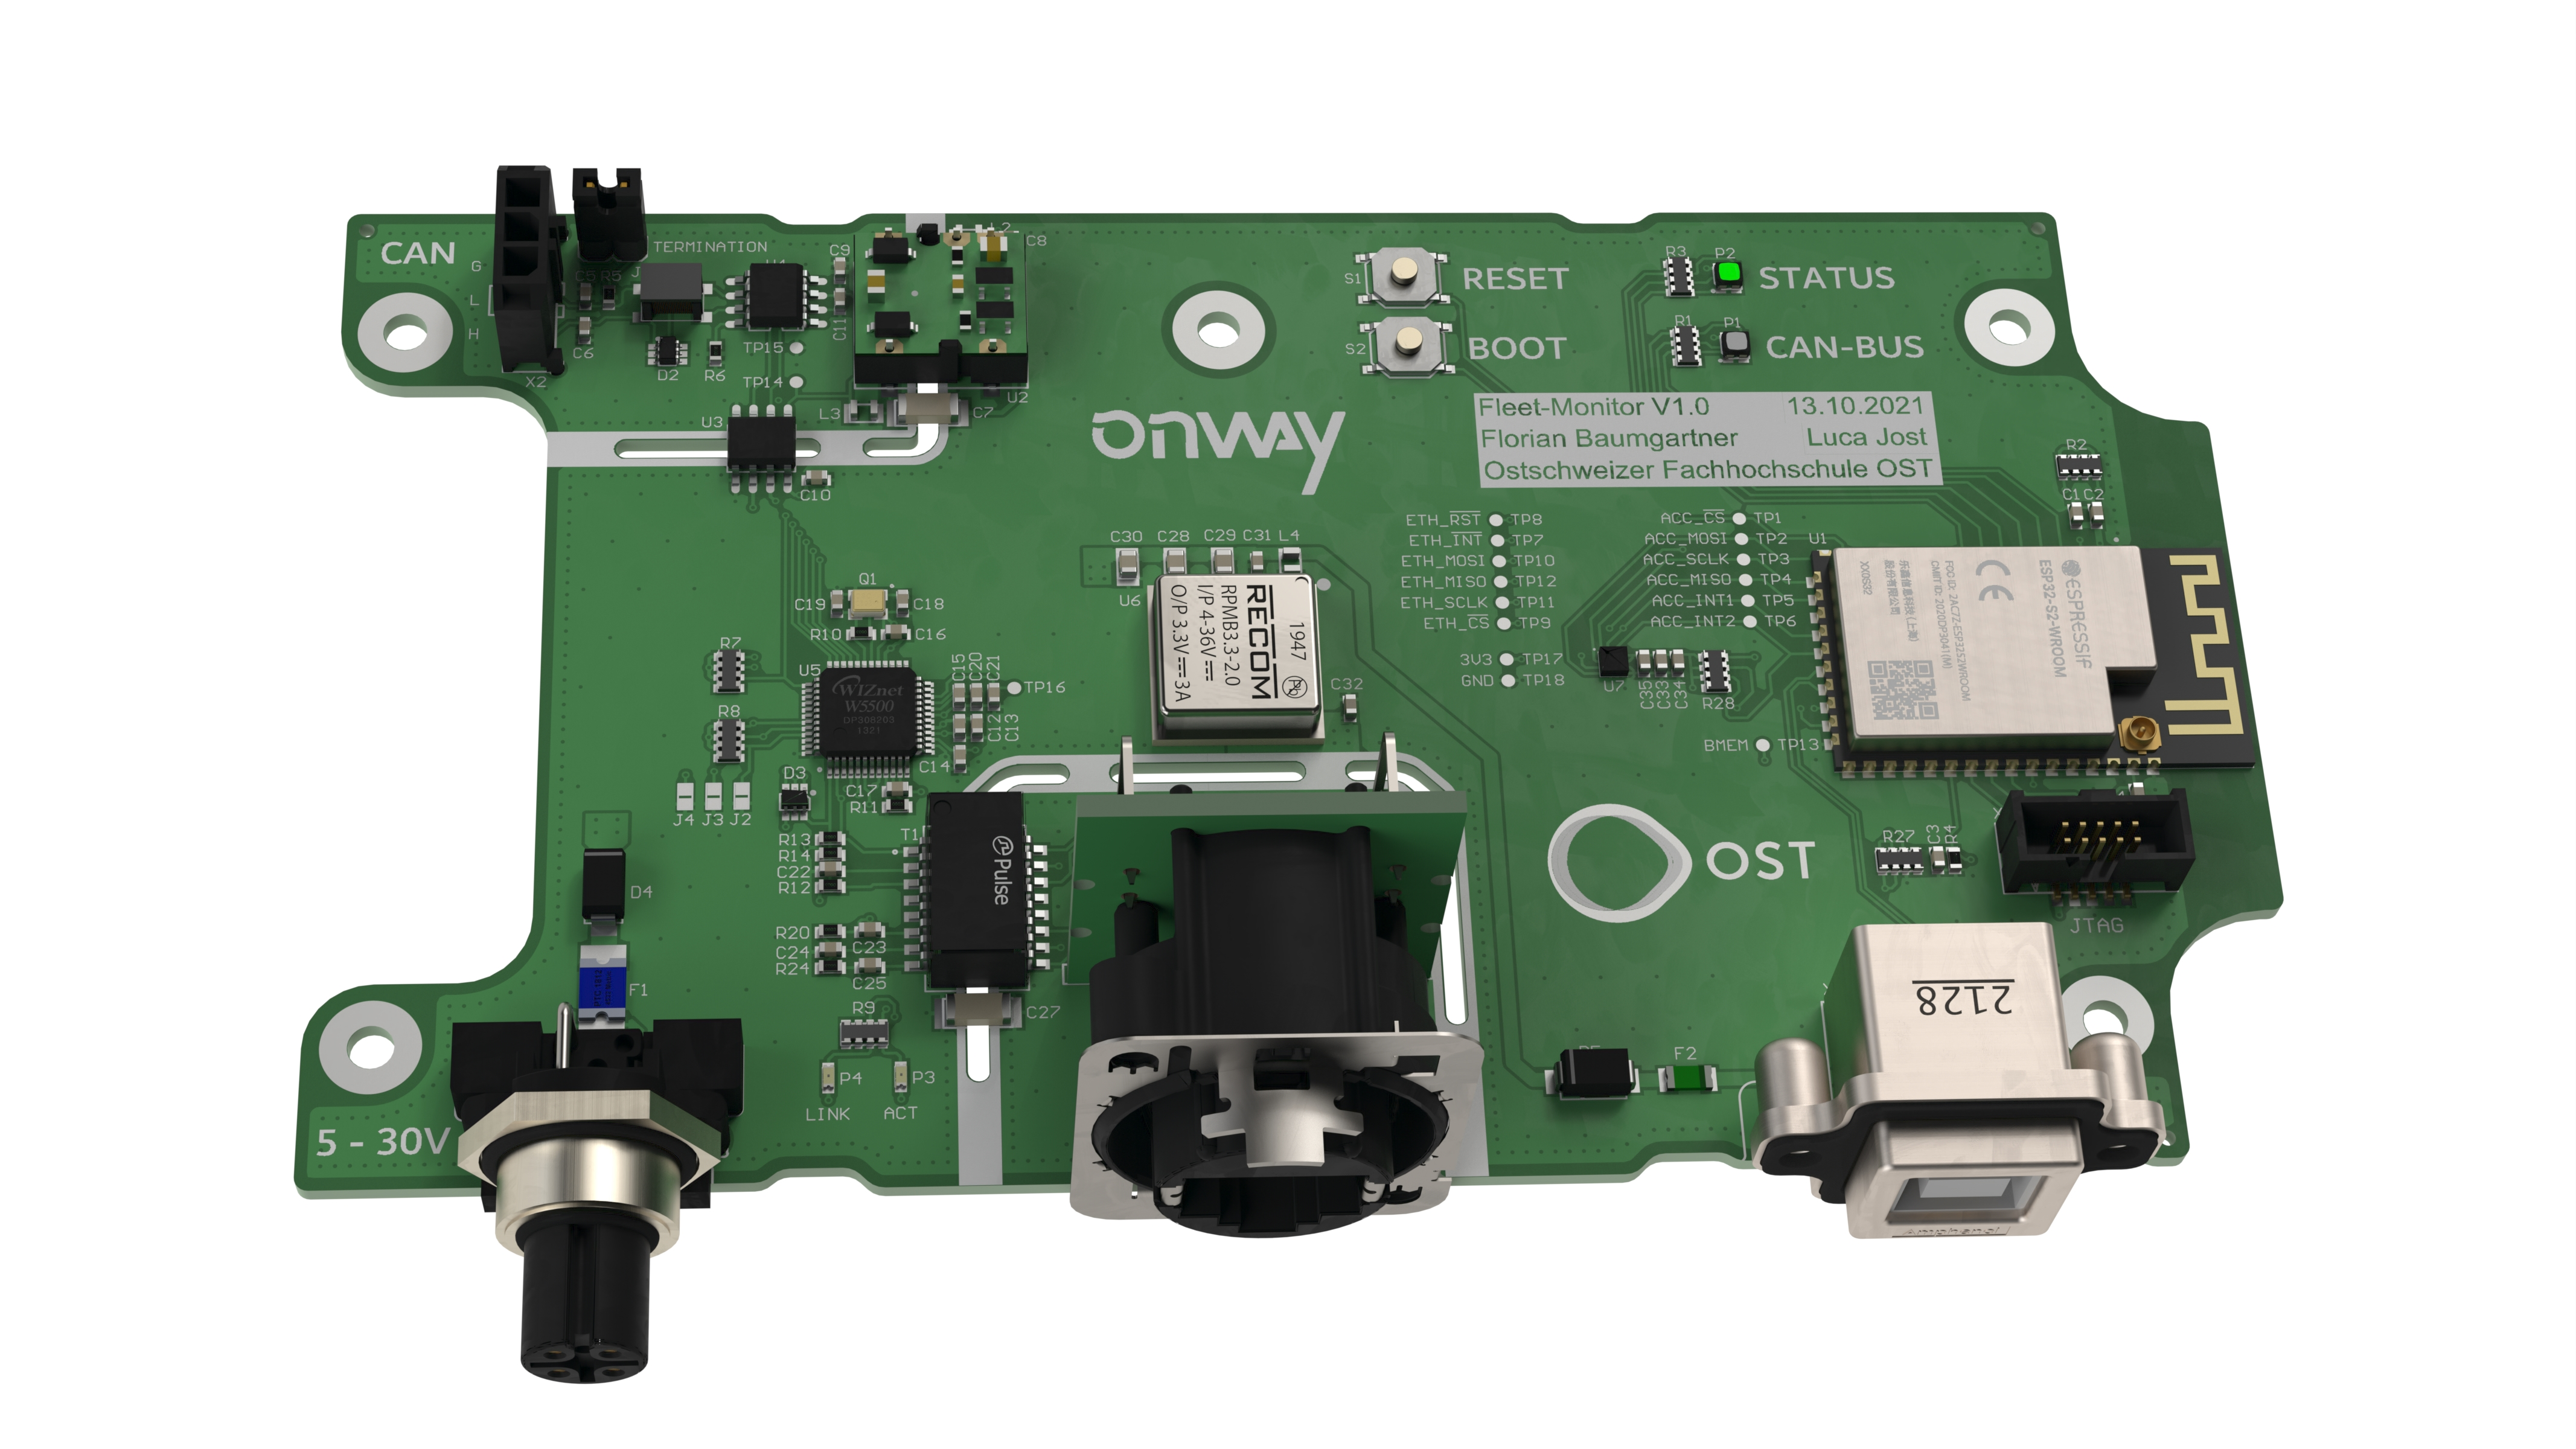
\includegraphics[height=10.0cm]{images/fleet-monitor-rendering-pcb}
	\caption{Assembled PCB 3D-Render}
	\label{fig:fleet-monitor-rendering-pcb}
\end{figure}
\newpage

\subsection{Power Management}
The device can be powered ether by the \acrshort{usb}-Interface or an external DC power source. Both supply options are internally connected through Schottky diodes and provide a seamless switch-over. If both supply sources provide power at the same time, the external one gets preferred.\newline
The \acrfull{usb} Interface fulfills all guidelines of the \acrshort{usb} specifications in terms of power consumption. Therefor it is guaranteed, that the maximal current of 500 mA is not exceeded. In case of failure, a resettable \acrshort{ptc} Poly-fuse protects the power source of potential over current.\newline
The external power source accepts a voltage range from 9 V to 28 V and is protected against wrong polarization and short circuit. As a suitable connector, the industry standard M12 (5 Pin) type has been chosen. It fulfils the IP67 rating and is highly robust against accidental disconnection due to its threaded coupling. In addition it is used in a wide variety of applications, resulting in great availability. The pin-out consists of pin 1 and 2 used for the positive input and pins 3 to 5 for ground. This has the advantage, that matching connectors with a different amount of pins (e.g. 2-pin connector) can be used as well.\newline
The core of the power management unit is based on a Recom DC-DC converter of the RPMB-2.0 series. The very compact design, great performance and fairly low price offers an optimal solution.\newline
The total power consumption of the device is in average around 1.5 W.

\bigskip
\begin{figure}[h!]
	\centering
	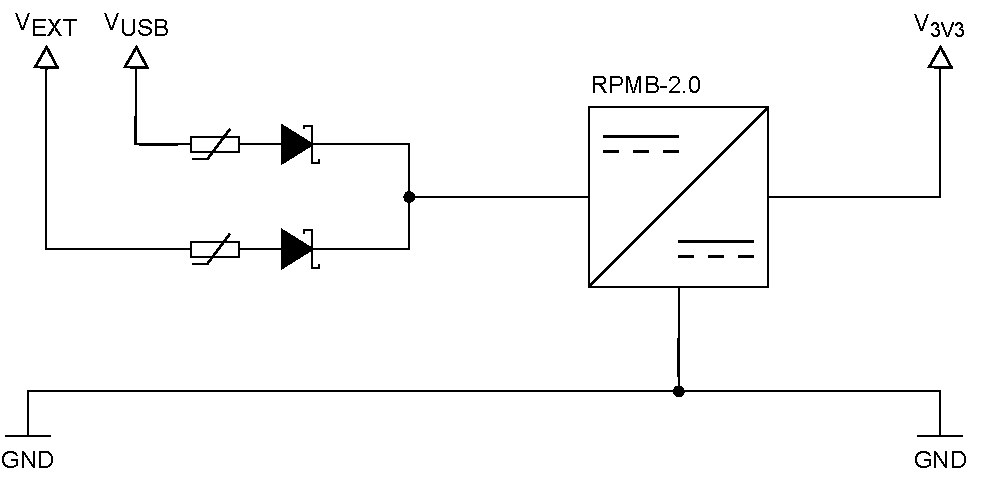
\includegraphics[height=5cm]{images/power}
	\caption{Simplified Power Management}
	\label{fig:simplified-power}
\end{figure}
\newpage

\subsection{ESP32-S2}
The choice of a suitable micro controller is crucial in the design of an embedded system. Several factors were carefully considered and key requirements have been set, such as:

\begin{itemize}
		\item Integrated Wi-Fi subsystem and \acrshort{rf} front-end
		\item System performance: CPU speed, memory and peripherals
		\item Native \acrshort{usb} 2.0 Interface
		\item Physical package and pin count
		\item Availability (especially in an ongoing worldwide chip-shortage)
\end{itemize}

The Espressif's \gls{esp32} \acrfull{soc} family satisfies all listed requirements and is in addition advertised as a low cost solution.\newline
To reduce design complexity and production cost, the ESP32-S2 has been embedded as a solder-on module of the type ESP32-S2-WROOM-I. This module has the advantage of containing the RF front-end inclusive an integrated \acrshort{pcb} antenna as well as a 4 MB \acrshort{spi} flash chip.

%\medskip
\begin{figure}[h!]
	\centering
	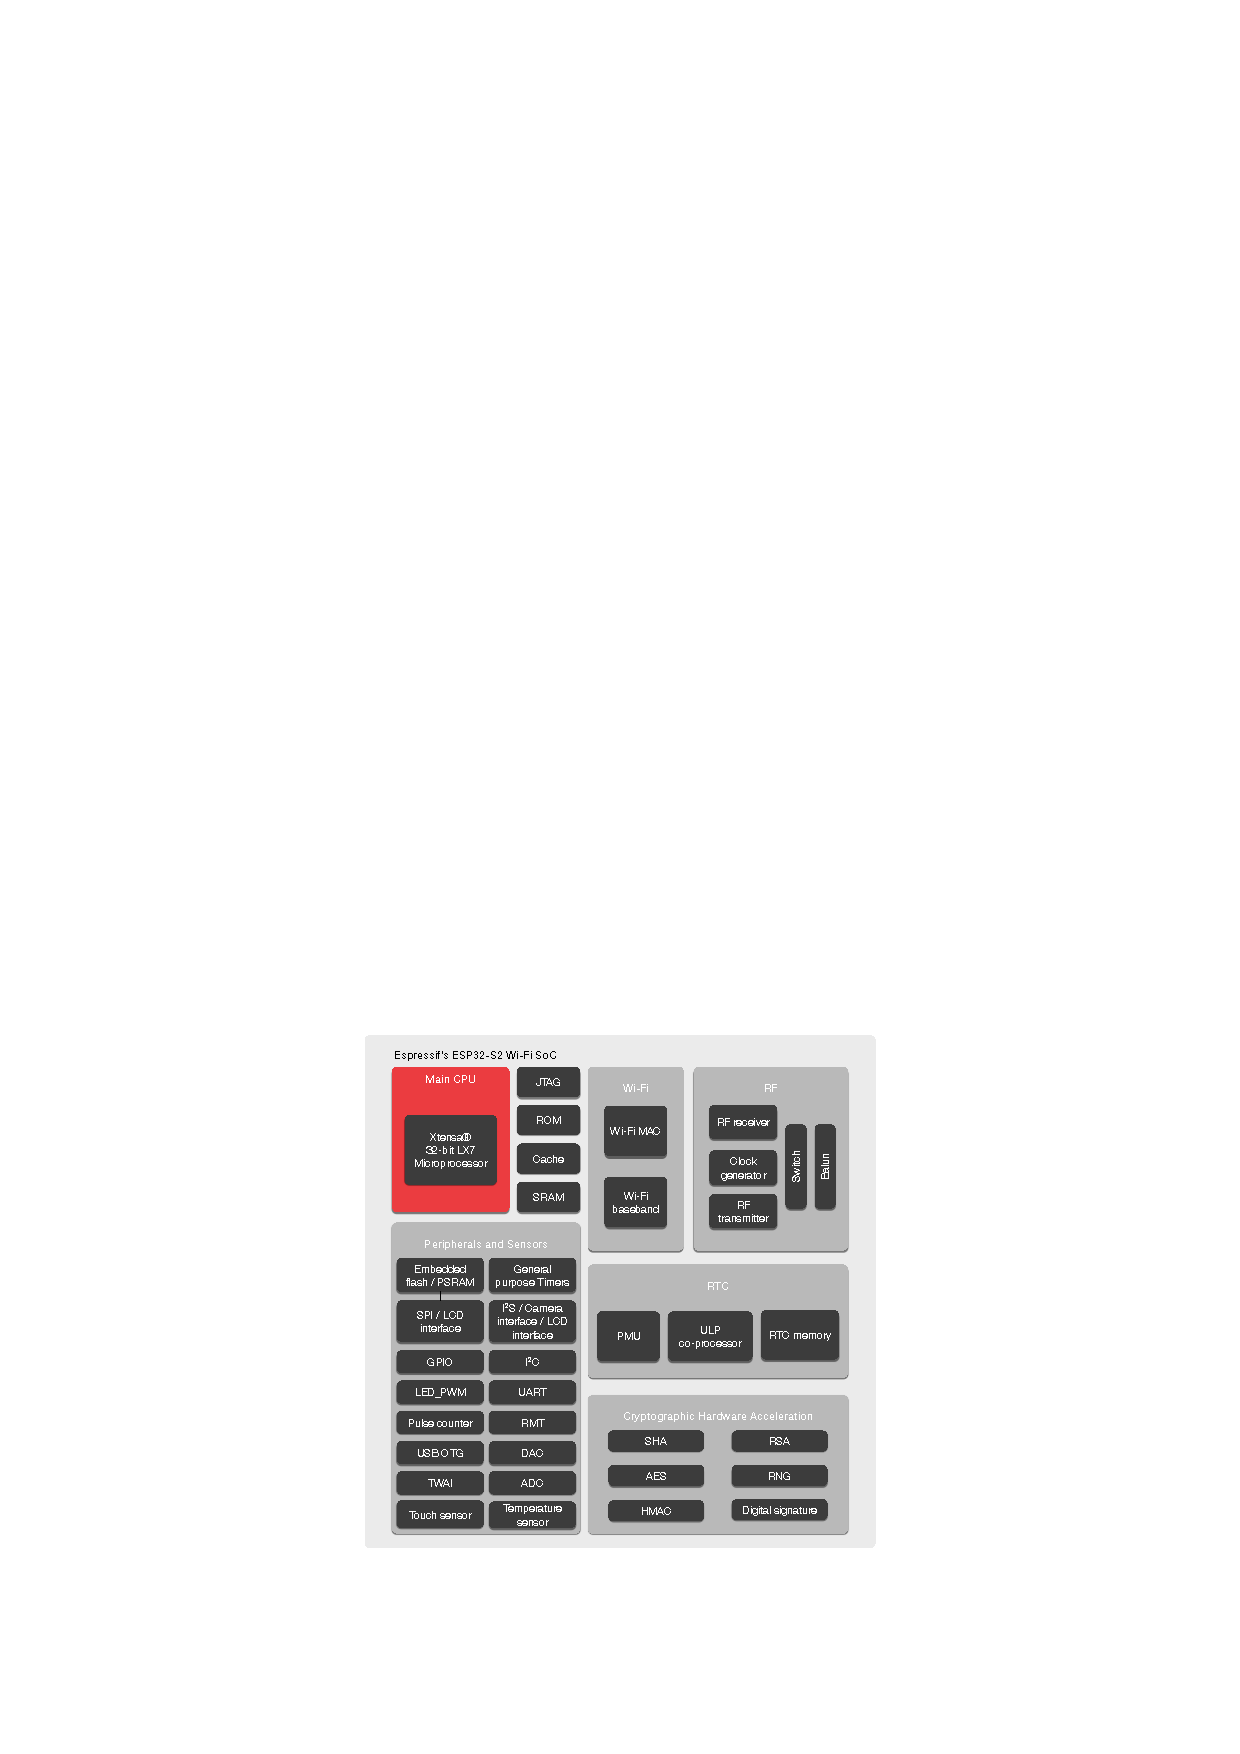
\includegraphics[height=9cm]{images/esp32-s2_block_diagram}
	\caption{ESP32-S2 Block Diagram}
	\vspace{-1.4ex}
	\caption*{\textbf{Source:} ESP32-S2 Datasheet \cite{esp32-s2_datasheet}}
	\label{fig:esp32-s2_block_diagram}
\end{figure}

The \acrshort{soc} can be programmed ether by \acrshort{jtag} and a suitable programmer (e.g. Espressif's ESP32-Prog) or conveniently over the integrated \acrshort{usb}-Interface.\newline
For uploading code via the \acrshort{usb}-Interface, the ESP32-S2 has to be set in to the device firmware update mode. This can be achieved by pressing the boot button while the device is booting (e.g. after powering on or a reset). If the boot button is not accessible, the user can force the device to enter the \acrshort{dfu} mode by setting a flag in the system configuration. This procedure gets further explained in the user manual section.
\newpage

\subsection{Ethernet Interface}
In order to connect the device to a host server, an Ethernet interface was added.

\begin{figure}[h!]
	\centering
	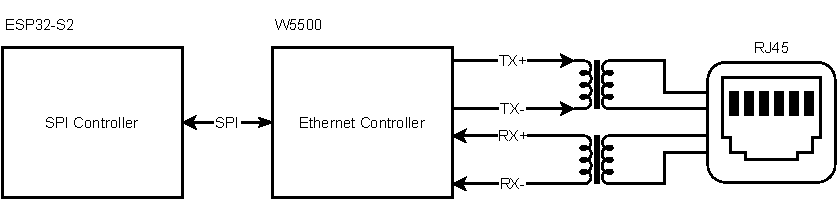
\includegraphics[height=3.0cm]{images/eth_interface}
	\vspace{0.2cm}
	\caption{Simplified Ethernet Interface}
	\label{fig:eth-interface}
\end{figure}

\subsubsection{Controller}
The Ethernet interface utilizes a WIZNet W5500 Ethernet controller chip with an integrated \acrshort{phy} and \acrshort{tcp/ip} stack. It is capable of transmission speeds of 10 or 100 MBit/s. The chip is connected through \acrshort{spi} with the main processing unit (\gls{esp32}).

\subsubsection{Isolation}
The IEEE standard 802.3 specifies a 1500 V\textsubscript{RMS} isolation barrier between the Ethernet PHY Chip and the cable. To comply with these requirements a pulse transformer was used to magnetically couple the data lines between the connector and the chip. Additionally a ground clearance of 3 mm was chosen to avoid arc-over or tracking between electrical conductors as seen in Figure \ref{fig:eth-pcb}. 

\begin{figure}[h!]
	\centering
	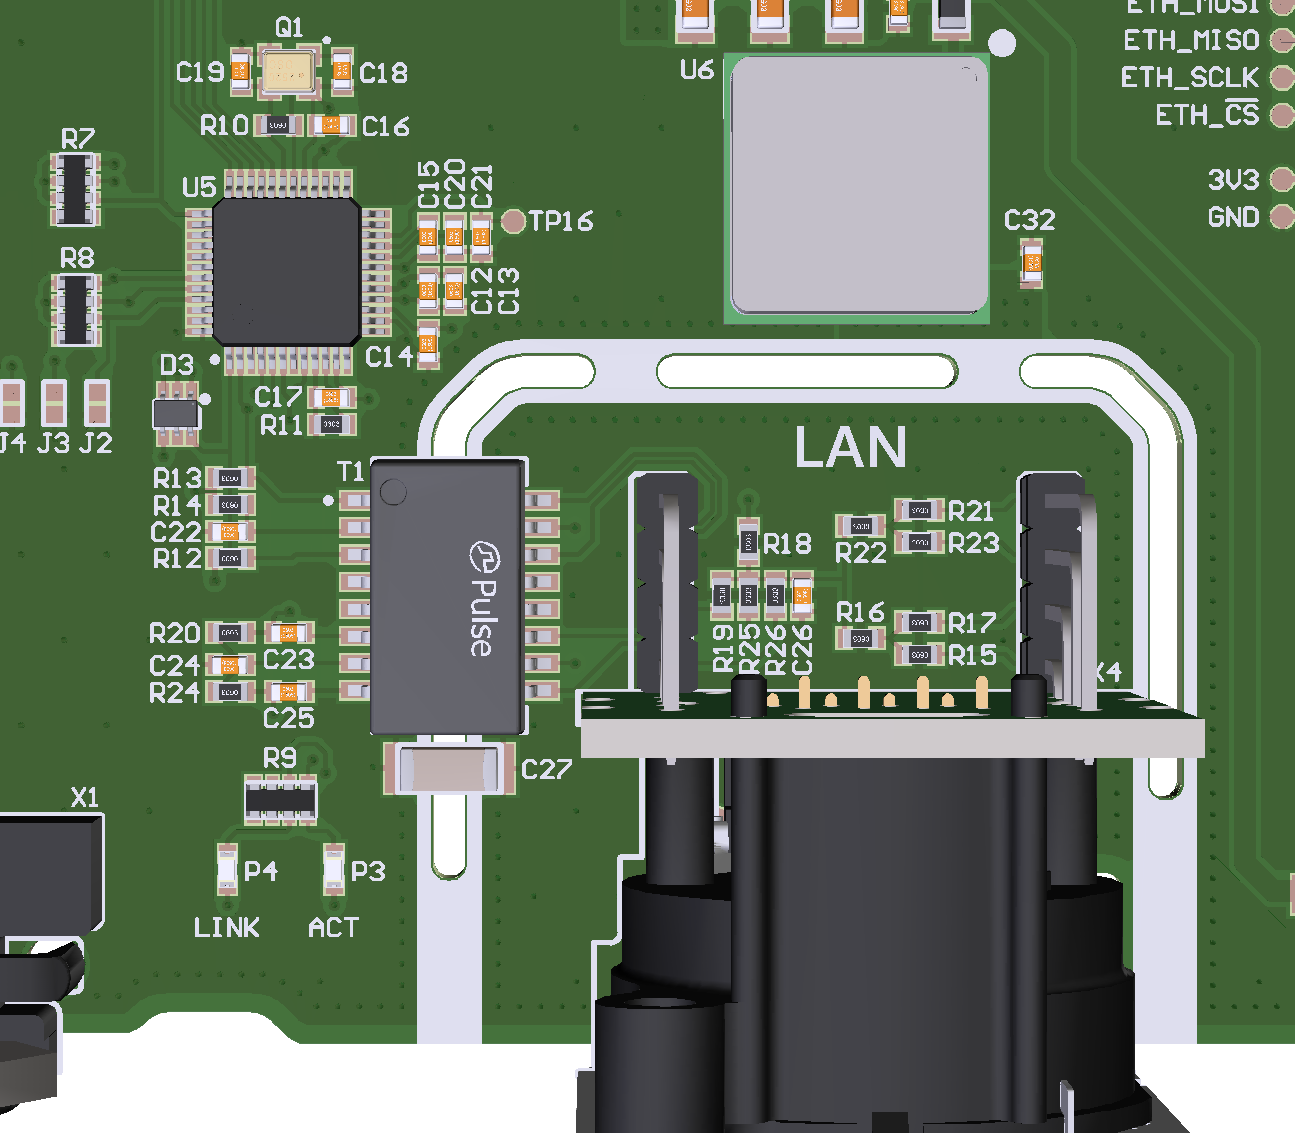
\includegraphics[height=8.5cm]{images/eth-pcb}
	\vspace{0.2cm}
	\caption{PCB view of Ethernet Interface}
	\label{fig:eth-pcb}
\end{figure}
\newpage

\subsubsection{Connector}
The etherCON RJ45 is a lockable connector system, it was chosen for its rugged design and water resistance. This connector system is often used in industrial applications, e.g. in the event industry. The receptacle accepts regular RJ45 plugs as well, but the use of proper etherCON connectors is recommended.

\begin{figure}[h!]
	\centering
	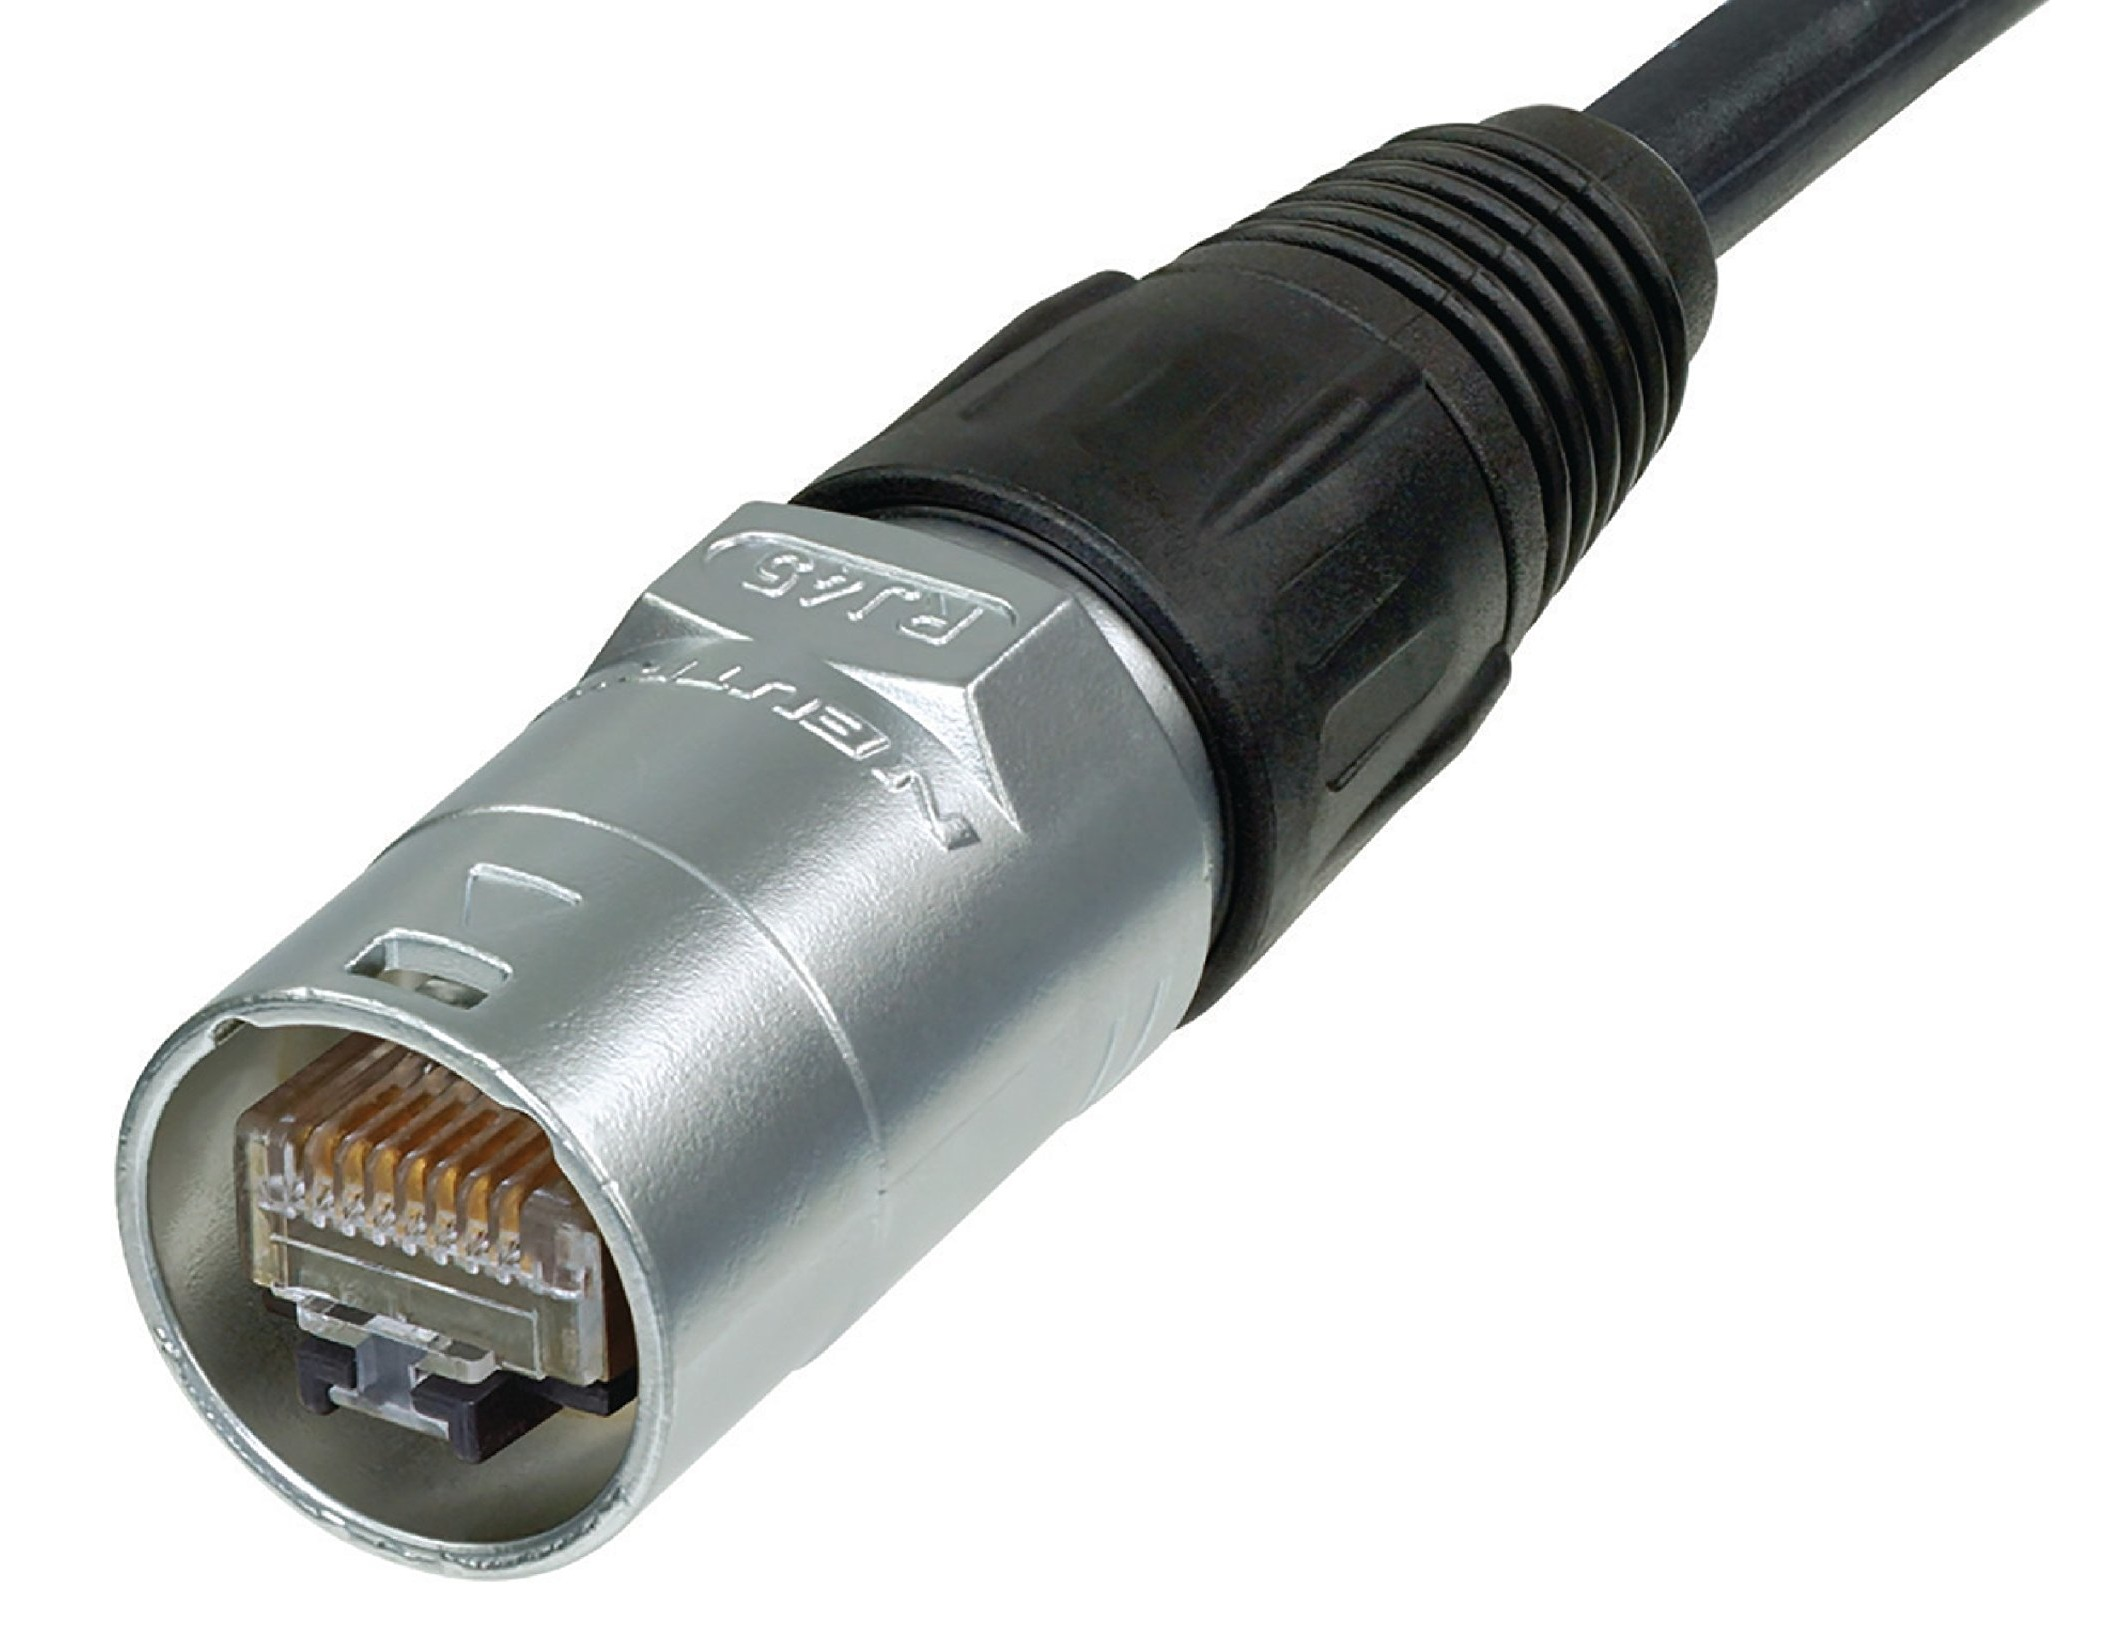
\includegraphics[height=6.5cm]{images/ethercon.jpg}
	\caption{etherCON Connector}
	\vspace{-1.4ex}
	\caption*{\textbf{Source:} Neutrik etherCON Connector NE8MX6 \cite{neutrik-ethercon}}
	\label{fig:neutrik-ethercon}
\end{figure}


\subsection{CAN-Bus Interface}
The \acrfull{twai} is a real-time serial communication protocol suited for automotive and industrial applications. It is compatible with CAN bus frames following the ISO11898-1 standard. The ESP32-S2 contains a \acrshort{twai} controller that can be configured to communicate on a CAN bus via an external transceiver.

\begin{figure}[h!]
	\centering
	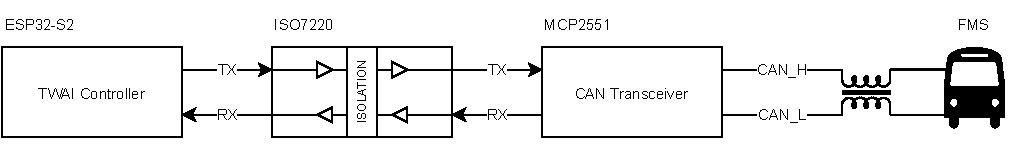
\includegraphics[height=2.0cm]{images/can-interface}
	\caption{Simplified CAN Interface}
	\label{fig:can-interface}
\end{figure}

\subsubsection{Transceiver}
The data lines are translated using a CAN transceiver from Microchip (MCP2551). The role of the transceiver is to drive and detect data to and from the bus. It converts the single-ended logic used by the controller to the differential signal transmitted over the bus. The MCP2551 device provides transmit and receive capabilities and is fully compatible with the ISO-11898 standard.
\newpage

\subsubsection{Isolation}
A dual-channel digital isolator (ISO7221BDR) was used in conjunction with an isolated DC/DC converter from Recom (R1SX-3.305/H). These devices block high voltage and isolate grounds, as well as prevent noise currents on a data bus or other circuits from entering the local ground and interfering with or damaging sensitive circuitry.

\begin{figure}[h!]
	\centering
	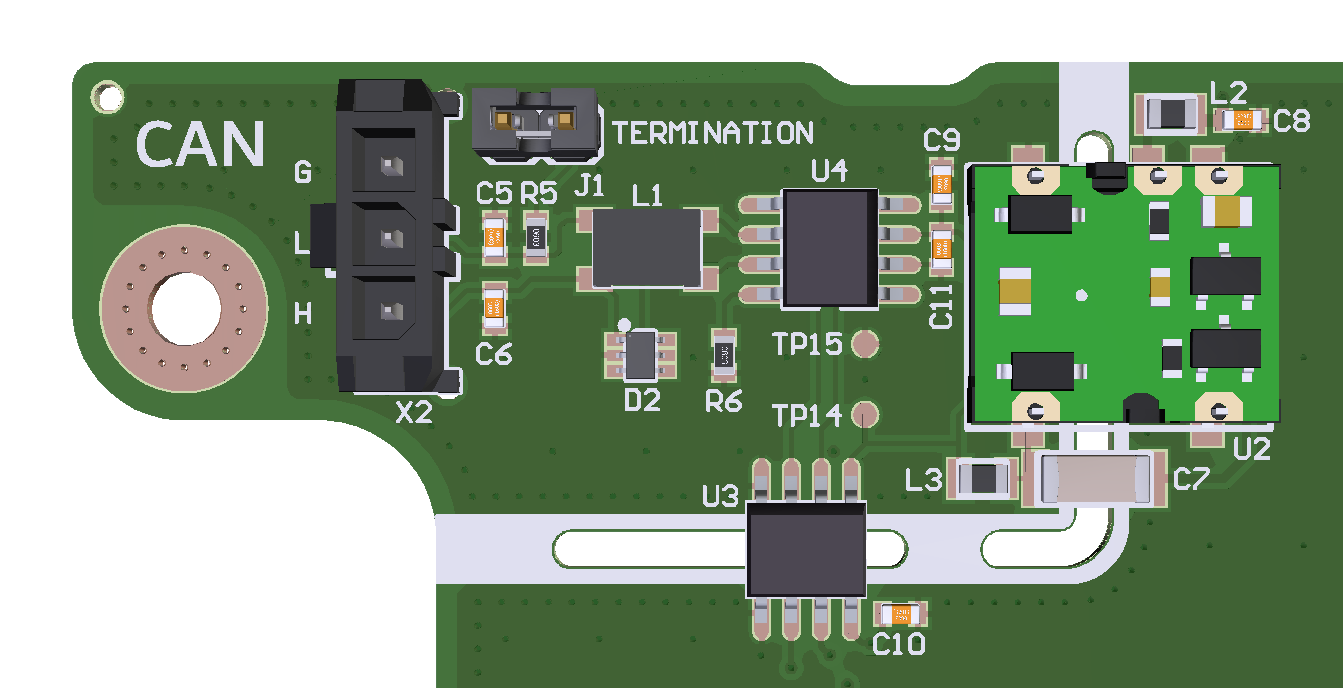
\includegraphics[height=4.5cm]{images/can-pcb}
	\caption{PCB view of CAN interface}
	\label{fig:can-pcb}
\end{figure}

\subsubsection{Filtering}
A common mode choke as well as bypass capacitors were added to the differential signal lines. A common mode choke is an electrical filter that blocks high frequency noise common to two or more data or power lines while allowing the desired DC or low-frequency signal to pass. Common mode (CM) noise is typically radiated from sources such as radio signals, unshielded electronics, inverters and motors. Additionally matching capacitors on the CANH and CANL lines were added to enhance the immunity against electromagnetic interference. 

\subsubsection{Connector}
The FMS Standard specifies a DIN 72585 connector as the default physical interface. Since these connectors are only available for panel mount, an additional wire to board connector was selected. A Molex Micro-Fit 3.0 was chosen because its widely available and being used in lots of applications.

\subsubsection{Termination}
In addition the FMS Standard specifies a 120$\Omega$ CAN termination resistor to be added on the monitor side. To fulfill this requirement and to make it compatible with system that do not need that resistor, a jumper was added to enable/disable the termination.   

\subsection{Accelerometer}
By request of the industry partner an accelerometer was added to gather additional data. The LIS2DH12 is an ultra-low-power high-performance three-axis linear accelerometer with digital I2C/SPI serial interface output. The sensor has user-selectable scales of ±2g up to ±16g and is capable of measuring accelerations with data rates from 1 Hz to 5.3 kHz. The sensor is connected through SPI to the ESP32.

\newpage
\section{Mechanical Design}
The automotive environment is known for its harsh conditions, such as vibrations, large temperature range and high humidity. The device must withstand those factors and should guarantee a long lifespan. The optimal selection of components, especially the connectors was key to satisfy the requirements and reach an IP67 rating.\newline
As a suitable case for the device, a poly-carbonate watertight enclosure with transparent lid has been chosen. The very robust construction creates an ideal protection for all electronic components.\newline
The case has been machined in the internal workshop of the university. The corresponding mechanical drawings have been made with SolidWorks 2020 and are attached in the appendix: \ref{Fleet-Monitor V1.0 Mechanical Drawing}

\medskip
\begin{figure}[h!]
	\centering
	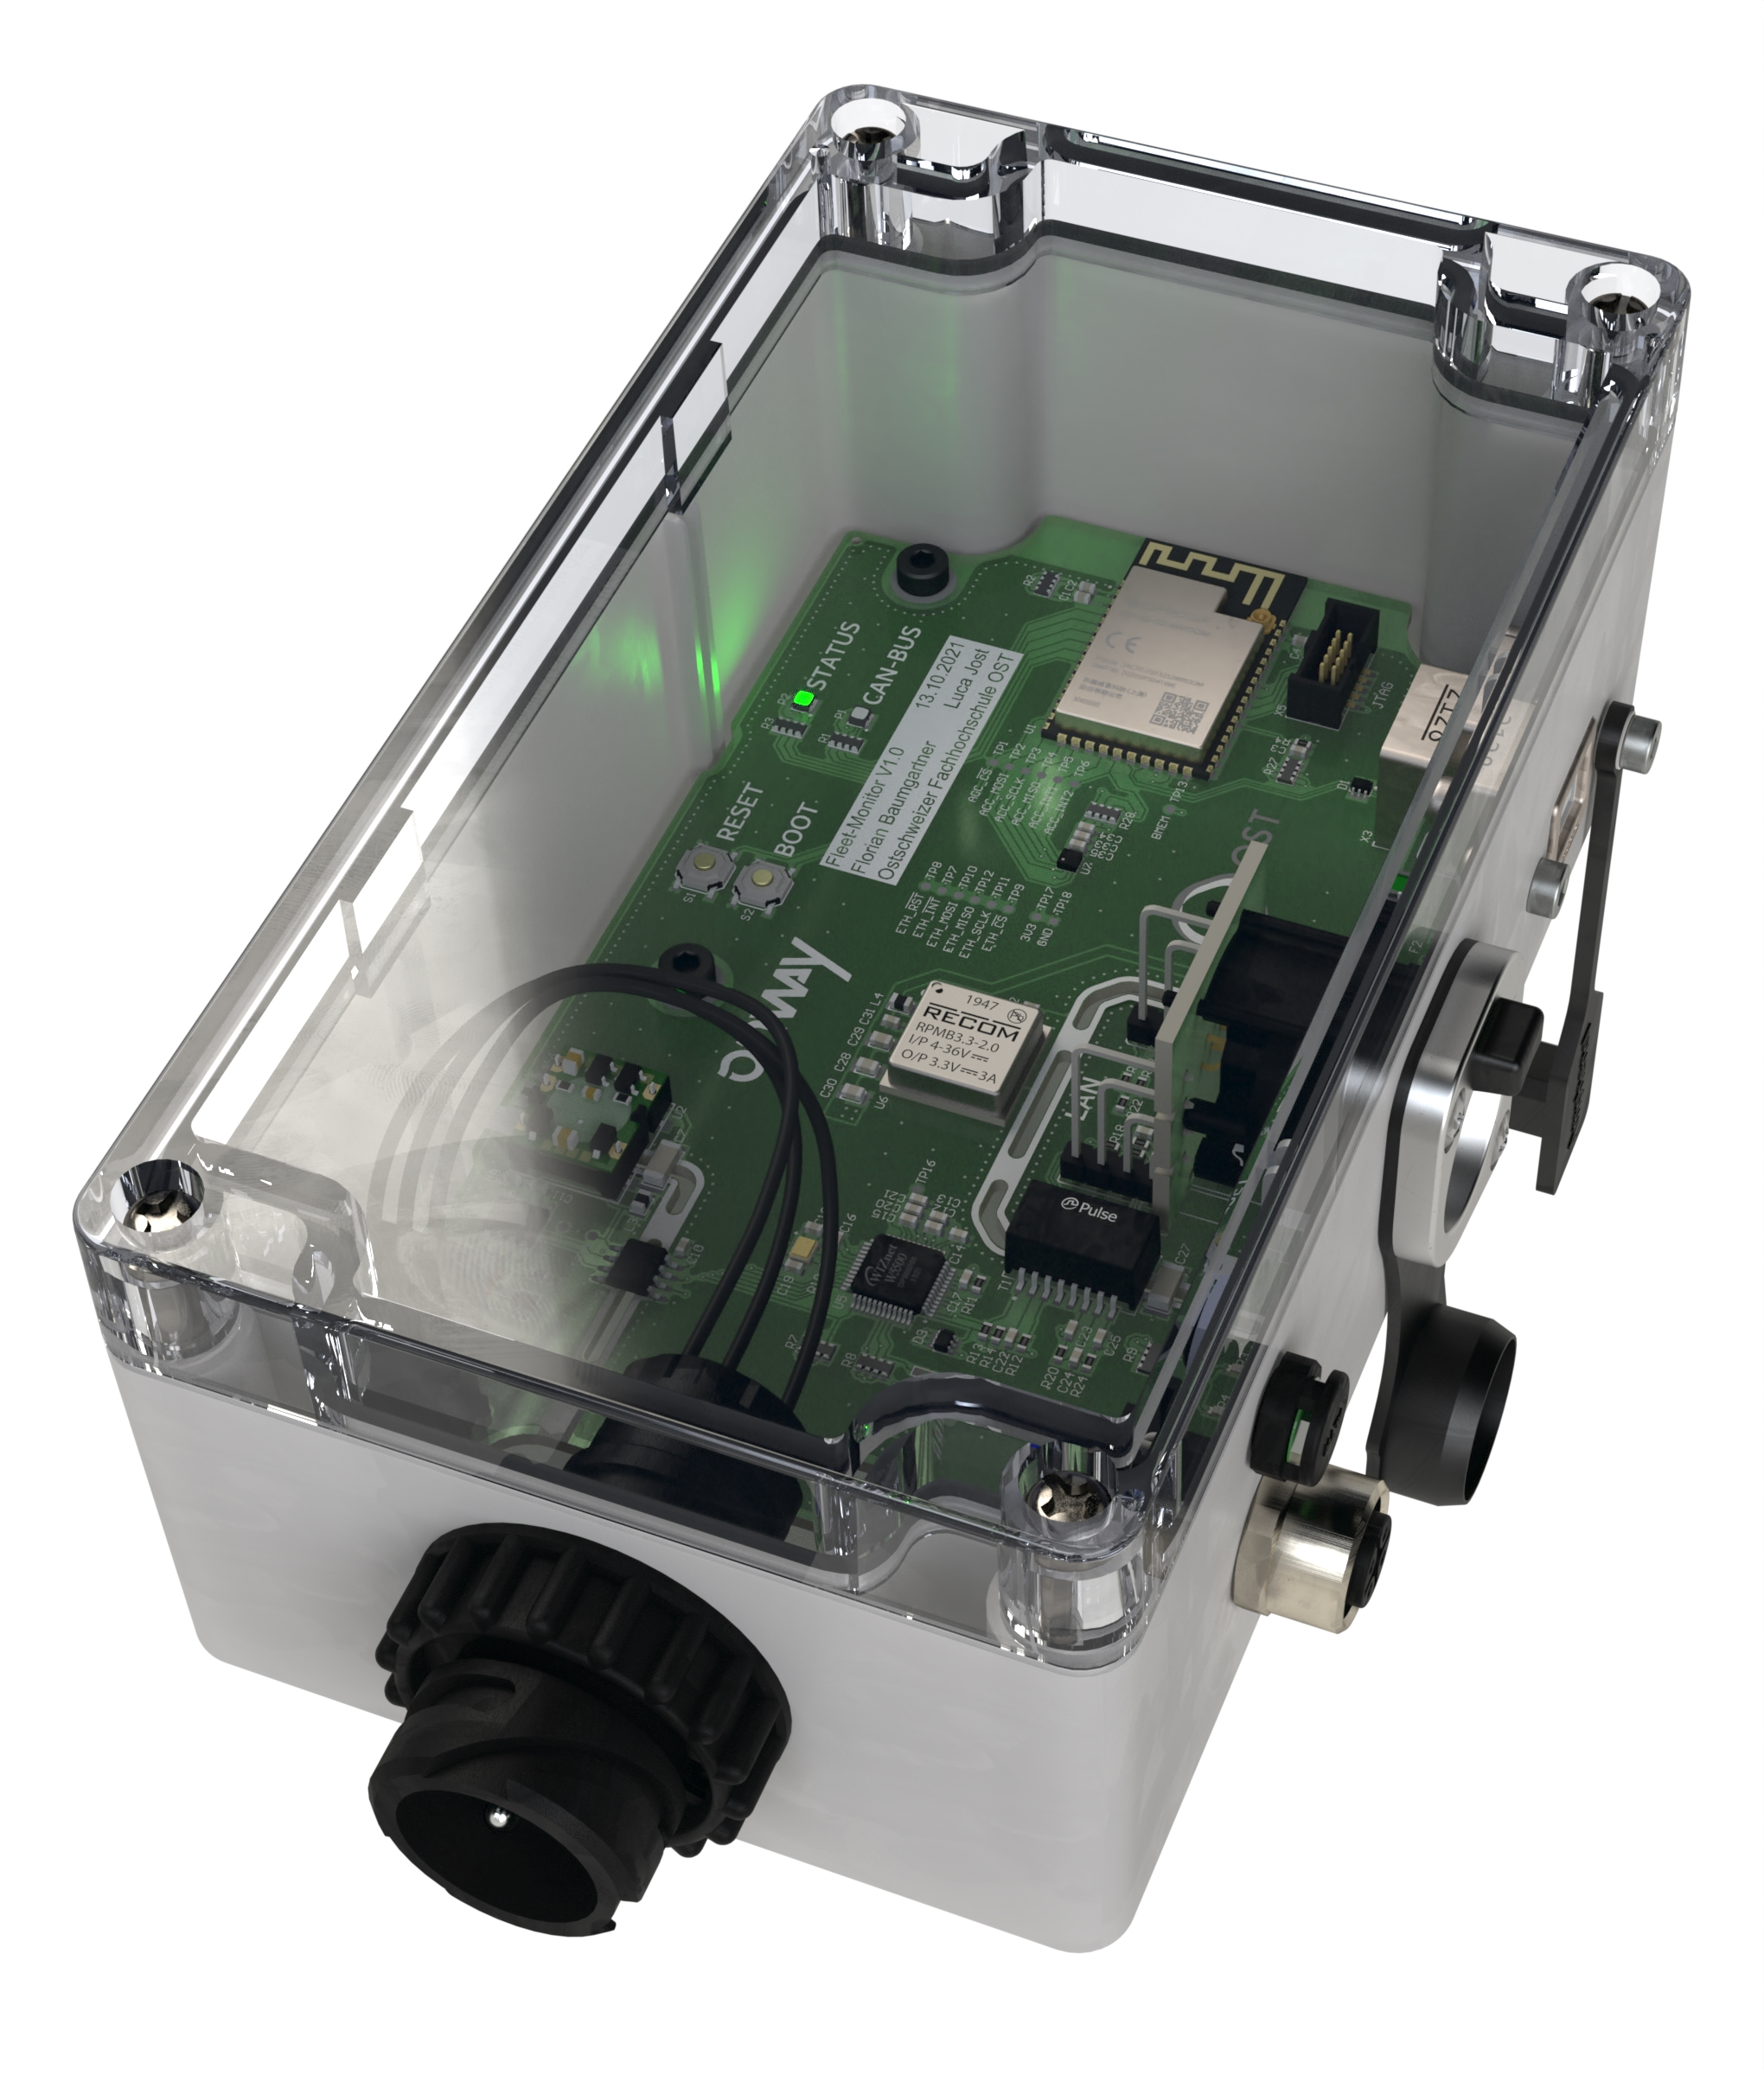
\includegraphics[height=16cm]{images/fleet-monitor-rendering}
	\caption{Final Product 3D-Render}
	\label{fig:fleet-monitor-rendering}
\end{figure}
\newpage

%% Section Firmware %%
\section{Firmware}
The firmware is written in C++ and is based on a combination of the Arduino and the ESP-IDF framework. As an IDE, Visual Studio Code with PlatformIO as an add-on has been used. This modern environment ensures rapid and effective development.\newline
FreeRTOS has been used as a real time operating system, which guarantees a reliable operation and handles multi-task operations even on a single core system.\newline
The Arduino framework offers extensive library support, especially for the \acrshort{usb} peripheral, file system and Ethernet interface. Due to the large community and the open source licensing, lots of individuals contribute bug-fixes and therefor increase the robustness of the software stack.

\subsection{File system}
The file system is an essential part of the device firmware. It enables accessing files stored on the internal \acrshort{spi}-Flash chip as well as creating an interface for additional libraries.
The flash chip has a memory capacity of 4 MB and is partitioned into four different sections. The size of each partition can be configured in the \textit{partitions\_custom.csv} file. Basically the memory is split into two partitions with ruffly the same size ($\approx$ 2 KB each) as a reasonable compromise between program memory and file system storage.

\begin{table}[h]
    \begin{tabular}{ | m{3.15cm} | m{3.15cm}| m{3.15cm} | m{3.15cm} |} 
      \hline
      \multicolumn{1}{|c|}{\textbf{Name}} & \multicolumn{1}{c|}{\textbf{Type}} & \multicolumn{1}{c|}{\textbf{Offset}} & \multicolumn{1}{c|}{\textbf{Size}}\\ \hline
      nvs & data & \codeword{0x009000} & 20K \\ \hline
      otadata & data & \codeword{0x00E000} & 8K \\  \hline
      app0 & app & \codeword{0x010000} & 2048K \\  \hline
      ffat & data & \codeword{0x210000} & 1984K \\  \hline
    \end{tabular}
    \caption{\label{tab:Flash-Partitions}SPI-Flash Partitions}
\end{table}

To provide a sufficient set of features, multiple libraries had to be used. Most of them are created by Adafruit Industries under \acrshort{mit} licensing. \newline
As a low-level \acrshort{spi}-Flash chip driver, the \codeword{Adafruit SPIFlash} library has been used. It handles the communication over the physical interface and provides access to the file system library named  \codeword{SdFAT}. The type of file system is \acrshort{fat}, which has the advantage of being compatible with most modern operating systems (Windows/Linux/Mac OS). Figure \ref{fig:file_system_stack} shows an overview of all utilized core library and how they are dependent.

\bigskip
\begin{figure}[h!]
	\centering
	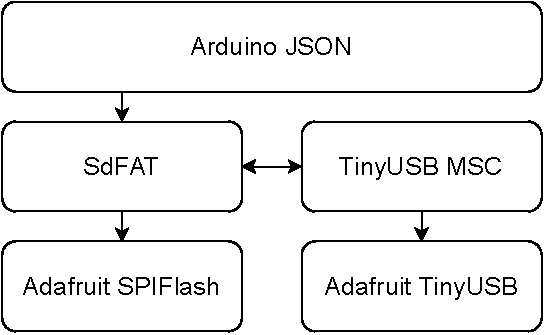
\includegraphics[height=5.2cm]{images/file_system_stack.pdf}
	\caption{USB and File System Library Stack}
	\label{fig:file_system_stack}
\end{figure}
\newpage


\subsection{USB Mass Storage Device}
\acrshort{usb} is known to be a very complex interface, however it provides lots of comport to an end-user. To enable \acrshort{usb} support on an embedded system, several layers of software are needed. Fortunately the open source project called TinyUSB supports the ESP32-S2 \acrshort{soc} family. This very comprehensive software stack supports the \acrshort{usb} \acrfull{msc} protocol.
As a result, the device acts just like a regular \acrshort{usb} Flash drive and provides seamless file access to any host computer. \newline
To pack all setup and configuration functions of the mentioned libraries together, an utility library has been made. The \codeword{utils_init()} function checks if the \acrshort{spi}-Flash chip has already been correctly formatted, if this is not the case, an automatic formatting procedure gets executed. In this process, a disk label can be set with a maximal length of 8 characters, in this case: \codeword{MONITOR}. The code section below shows how those utility functions are called at the beginning of the program execution.

\bigskip
\colorlet{mygray}{black!30}
\colorlet{mygreen}{green!60!blue}
\colorlet{mymauve}{red!60!blue}
\begin{lstlisting}[backgroundcolor=\color{gray!10},  
                   basicstyle=\ttfamily,
                   columns=fullflexible,
                   breakatwhitespace=false,      
                   breaklines=true,                
                   captionpos=b,                    
                   commentstyle=\color{mygreen}, 
                   extendedchars=true,              
                   frame=single,                   
                   keepspaces=true,             
                   keywordstyle=\color{blue},      
                   language=c++,                 
                   numbers=none,                
                   numbersep=5pt,                   
                   numberstyle=\tiny\color{blue}, 
                   rulecolor=\color{mygray},        
                   showspaces=false,
                   showstringspaces=false,
                   showtabs=false,                 
                   stepnumber=5,                  
                   stringstyle=\color{mymauve},    
                   tabsize=2,                      
                   title=\lstname,
                   frame=none,
                   xleftmargin = 1cm,
                   framexleftmargin = 1em]
utils_init("MONITOR");  // Initialize peripherals and file system
utils_systemConfig("system.json");   // Load system configuration
utils_startMsc();       // Start USB mass storage controller
\end{lstlisting}

In addition to the \acrshort{usb} \acrshort{msc} protocol, a \acrfull{cdc} has been set up. This creates a \acrfull{vcp} over which the host computer can gain debug information from the device. \newline
After initializing the \acrshort{usb}-Interface and file system, the device configuration is loaded from the locally stored \acrshort{json}-File, more details in the section \ref{System Configuration}.

\subsection{JSON Parser Library} \label{JSON Parser Library}
Due to the frequently usage of the \acrshort{json}-File format in this project, using an advanced software library was key to accelerate the development process. \\
In this case, the open source ArduinoJSON library has been used. It makes use of modern C++14 syntax and is optimized for small architectures like micro controllers. In addition, support for static and dynamic data allocation simplifies the serializing and deserializing of files without a predefined size. This is especially useful for parsing incoming data over the Ethernet interface. \\[0.5em]
The following code snippet shows how to iterate over a list of elements. If a matching entry has been found, the corresponding name gets returned as a char string. This example illustrates how intuitive the the iterating feature is applied and how fields can dynamically be manipulated.

\bigskip
\colorlet{mygray}{black!30}
\colorlet{mygreen}{green!60!blue}
\colorlet{mymauve}{red!60!blue}
\begin{lstlisting}[backgroundcolor=\color{gray!10},  
                   basicstyle=\ttfamily,
                   columns=fullflexible,
                   breakatwhitespace=false,      
                   breaklines=true,                
                   captionpos=b,                    
                   commentstyle=\color{mygreen}, 
                   extendedchars=true,              
                   frame=single,                   
                   keepspaces=true,             
                   keywordstyle=\color{blue},      
                   language=c++,                 
                   numbers=none,                
                   numbersep=5pt,                   
                   numberstyle=\tiny\color{blue}, 
                   rulecolor=\color{mygray},        
                   showspaces=false,
                   showstringspaces=false,
                   showtabs=false,                 
                   stepnumber=5,                  
                   stringstyle=\color{mymauve},    
                   tabsize=2,                      
                   title=\lstname,
                   frame=none,
                   xleftmargin = 1cm,
                   framexleftmargin = 1em]
for (JsonVariant value : doc["frames"].as<JsonArray>())
{
  if (strncmp(value["pgn"].as<const char*>(), pgnStr, 4) == 0)
  {
    return value["name"].as<const char*>();
  }
}
\end{lstlisting}


\newpage

\subsection{System Configuration} \label{System Configuration}
The system configuration is defined in a \acrshort{json}-File called \codeword{system.json}, stored in the root directory of the file system. This file gets read and parsed on every startup or reset. The following parameter can be configured:

\begin{table}[h]
    \hfuzz=23.0pt
    \begin{tabular}{ | p{2.8cm} | p{1.3cm} | p{5.9cm} | p{2.7cm} |}
      \hline
      \multicolumn{1}{|c|}{\textbf{Parameter}} & \multicolumn{1}{c|}{\textbf{Type}} & \multicolumn{1}{c|}{\textbf{Description}} & \multicolumn{1}{c|}{\textbf{Example}}\\ \hline
      \codeword{ssid} & string & \acrshort{ssid} of \acrfull{ap} & \codeword{"network"} \hfuzz=3.0pt  \\ \hline
      \codeword{password} & string & Password of \acrshort{ap} * & \codeword{"secret"} \\ \hline
      \codeword{connection} & string & Preferred connection type: \newline\codeword{[auto, lan, wlan]}  & \codeword{"auto"} \\ \hline
      \codeword{config} & string & Location of config file: \newline\codeword{[local, remote]} & \codeword{"remote"} \\ \hline
      \codeword{host_ip} & string & IP Address of host server & \codeword{"10.3.141.1"} \\ \hline
      \codeword{host_port} & integer & Port of host server & \codeword{8080} \\ \hline \hfuzz=10.0pt 
      \codeword{overwrite_file} & boolean & Overwrite locally stored config file with remotely downloaded version & \codeword{True} \\ \hline
      \codeword{bootloader} & boolean & Restart device in \acrshort{dfu} mode ** & \codeword{False} \\ \hline
    \end{tabular}
    \caption{\label{tab:System-Configuration}System Configuration Parameter Description}
\end{table}

* Password field gets cleared after config file has been loaded due to security reasons.
** If set \codeword{True}, device reboots immediately in \acrshort{dfu} mode and field gets reset to \codeword{False}.

\subsection{Frame Filter Configuration} \label{Frame Filter Configuration}
The configuration of the \acrshort{fms}-Frame filter is based on a specific \acrshort{json}-File called \codeword{config.json}, which is as well stored in the root directory of the file system. In addition the filter configuration gets remotely downloaded from the host server if the \codeword{config} parameter in the system configuration is set to \codeword{remote}. This has the advantage of adjusting parameters in real time and therefore conveniently manage the data stream.
Basically the \acrshort{json}-File consists two types of configuration parameters. First of all the general settings which describe how the data should be uploaded to the server: \\[0.3em]
\codeword{framename} enables or disables the transmission of the \acrshort{fms}-Packet name. Turning off this parameter, reduces the overall data upload size and thus minimizes network traffic. For debugging purpose, enabling this setting can help identifying \acrshort{fms}-Frames. \\[0.3em]
\codeword{unknownframes} enables or disables the transmission of unknown \acrshort{fms}-Packets, meaning frames that are not listed in the configuration settings. \\[0.3em]
The second part of the configuration file contains a look-up table with \acrshort{fms}-Frame information and filter settings in form of a list. The different filter types are further described in section \ref{FMS Frame Handler}. Each entry consists of multiple fields specified as followed:

\begin{table}[h!]
    \hfuzz=23.0pt
    \begin{tabular}{ | p{1.4cm} | p{2.2cm} | p{8.9cm} |} \hline
      \multicolumn{1}{|c|}{\textbf{Parameter}} & \multicolumn{1}{c|}{\textbf{Type}} & \multicolumn{1}{c|}{\textbf{Description}} \\ \hline 
      \codeword{pgn} & \acrshort{ascii}-HEX & \acrfull{pgn} as 4 digit number \hfuzz=3.0pt  \\ \hline
      \codeword{name} & string & Human friendly frame name \hfuzz=3.0pt  \\ \hline
      \codeword{active} & boolean & Transmission state, \codeword{False} means ignore frame type \hfuzz=3.0pt  \\ \hline
      \codeword{filter} & string & Filter type: \codeword{[nofilter, change, interval]} \hfuzz=3.0pt  \\ \hline
      \codeword{time} & integer & Max. interval time in [ms], field exists only if filter type is set to \codeword{interval} \hfuzz=3.0pt  \\ \hline
    \end{tabular}
    \caption{\label{tab:frame-parameter-description}Frame Filter Parameter Description}
\end{table}

%\newpage
The following example shows how the \acrshort{json}-File is structured. For better visibility some of the packet settings have been hidden.

\begin{table}[h!]
    \begin{center}
    \framebox{
        \begin{tabular}{p{0.0cm} p{0.1cm} p{0.1cm} p{0.1cm} p{7.0cm}}                                       \\[-0.5em]
        & \multicolumn{4}{l}{$\triangledown$ \texttt{JSON \{3\}}}                                           \\[0.3em]
        & & \multicolumn{3}{l}{\scalebox{0.8}{$\square$} \texttt{framename:\;\ \ \quad\textbf{True}}}       \\[0.3em]
        & & \multicolumn{3}{l}{\scalebox{0.8}{$\square$} \texttt{unknownframes:\;\textbf{False}}}           \\[0.3em]
        & & \multicolumn{3}{l}{$\triangledown$ \texttt{frames [34]}}                                        \\[0.3em]
        & & & \multicolumn{2}{l}{$\triangledown$ \texttt{0 \{4\}}}                                          \\[0.3em]
        & & & & \scalebox{0.8}{$\square$} \texttt{pgn:\;\ \quad\textbf{FEE9}}                               \\[0.3em]
        & & & & \scalebox{0.8}{$\square$} \texttt{name:\;\quad\textbf{Fuel Consumption: LFC}}               \\[0.3em]
        & & & & \scalebox{0.8}{$\square$} \texttt{active:\;\textbf{True}}                                   \\[0.3em]
        & & & & \scalebox{0.8}{$\square$} \texttt{filter:\;\textbf{nofilter}}                               \\[0.3em]
        & & & \multicolumn{2}{l}{$\triangledown$ \texttt{1 \{4\}}}                                          \\[0.3em]
        & & & & \scalebox{0.8}{$\square$} \texttt{pgn:\;\ \quad\textbf{FE6C}}                               \\[0.3em]
        & & & & \scalebox{0.8}{$\square$} \texttt{name:\;\quad\textbf{Tachograph: TCO1}}                    \\[0.3em]
        & & & & \scalebox{0.8}{$\square$} \texttt{active:\;\textbf{True}}                                   \\[0.3em]
        & & & & \scalebox{0.8}{$\square$} \texttt{filter:\;\textbf{interval}}                               \\[0.3em]
        & & & & \scalebox{0.8}{$\square$} \texttt{time:\;\ \ \textbf{100}}                                  \\[0.3em]
        & & & \multicolumn{2}{l}{$\triangledown$ \texttt{2 \{4\}}}                                          \\[0.3em]
        & & & & \scalebox{0.8}{$\square$} \texttt{pgn:\;\ \quad\textbf{FE4E}}                               \\[0.3em]
        & & & & \scalebox{0.8}{$\square$} \texttt{name:\;\quad\textbf{Door Control 1: DC1}}                 \\[0.3em]
        & & & & \scalebox{0.8}{$\square$} \texttt{active:\;\textbf{True}}                                   \\[0.3em]
        & & & & \scalebox{0.8}{$\square$} \texttt{filter:\;\textbf{change}}                                 \\[0.3em]
        & & & \multicolumn{2}{l}{$\triangledown$ \texttt{3 \{4\}}}                                          \\[0.3em]
        & & & & \scalebox{0.8}{$\square$} \texttt{pgn:\;\ \quad\textbf{FDA5}}                               \\[0.3em]
        & & & & \scalebox{0.8}{$\square$} \texttt{name:\;\quad\textbf{Door Control 2: DC2}}                 \\[0.3em]
        & & & & \scalebox{0.8}{$\square$} \texttt{active:\;\textbf{False}}                                  \\[0.3em]
        & & & & \scalebox{0.8}{$\square$} \texttt{filter:\;\textbf{nofilter}}                               \\[0.3em]
        & & & \multicolumn{2}{l}{$\triangledown$ \texttt{4 \{4\}}}                                          \\[0.3em]
        & & & & \scalebox{0.8}{$\square$} \texttt{pgn:\;\ \quad\textbf{FEEA}}                               \\[0.3em]
        & & & & \scalebox{0.8}{$\square$} \texttt{name:\;\quad\textbf{Vehicle Weight: VW}}                  \\[0.3em]
        & & & & \scalebox{0.8}{$\square$} \texttt{active:\;\textbf{True}}                                   \\[0.3em]
        & & & & \scalebox{0.8}{$\square$} \texttt{filter:\;\textbf{interval}}                               \\[0.3em]
        & & & & \scalebox{0.8}{$\square$} \texttt{time:\;\ \ \textbf{5000}}                                 \\[0.3em]
        & & & \multicolumn{2}{l}{$\rhd$ \texttt{5 \{4\}}}                                                   \\[0.3em]
        & & & \multicolumn{2}{l}{$\rhd$ \texttt{6 \{4\}}}                                                   \\[0.3em]
        & & & \multicolumn{2}{l}{...}                                                                       \\[0.3em]
        & & & \multicolumn{2}{l}{$\rhd$ \texttt{34 \{4\}}}                                                  \\[0.4em]
        \end{tabular}
    }
    \end{center}
\vspace{-0.3cm}
\caption{\label{fig:frame-configuration-example}Frame Filter Configuration Example}
\end{table}
\newpage

\subsection{Networking}  \label{Networking}
The Fleet-Monitor needs to communicate with a server to stream data, exchange the current time and read configuration data. 
\subsubsection{Connection}
The device can connect through WIFI or Ethernet with the host. Both interfaces utilize UDP to negotiate an IP address and the server IP can be configured through the system configuration. The device can be connected to both interfaces at the same time but only one is used to communicate with the server. 

The connection is checked every 5 seconds and works as follows. First the hardware status is checked, then the connection to a host and lastly if we received an IP address. The Ethernet interface is the prioritized communication method. It provides better data throughput and is less prone to errors than the over the air alternative. For example, if both interfaces received an IP address and are able to communicate with the server, Ethernet is used for the transmission. This is illustrated in Figure \ref{fig:connectin-tree} bellow.
\begin{figure}[!ht]
	\centering
	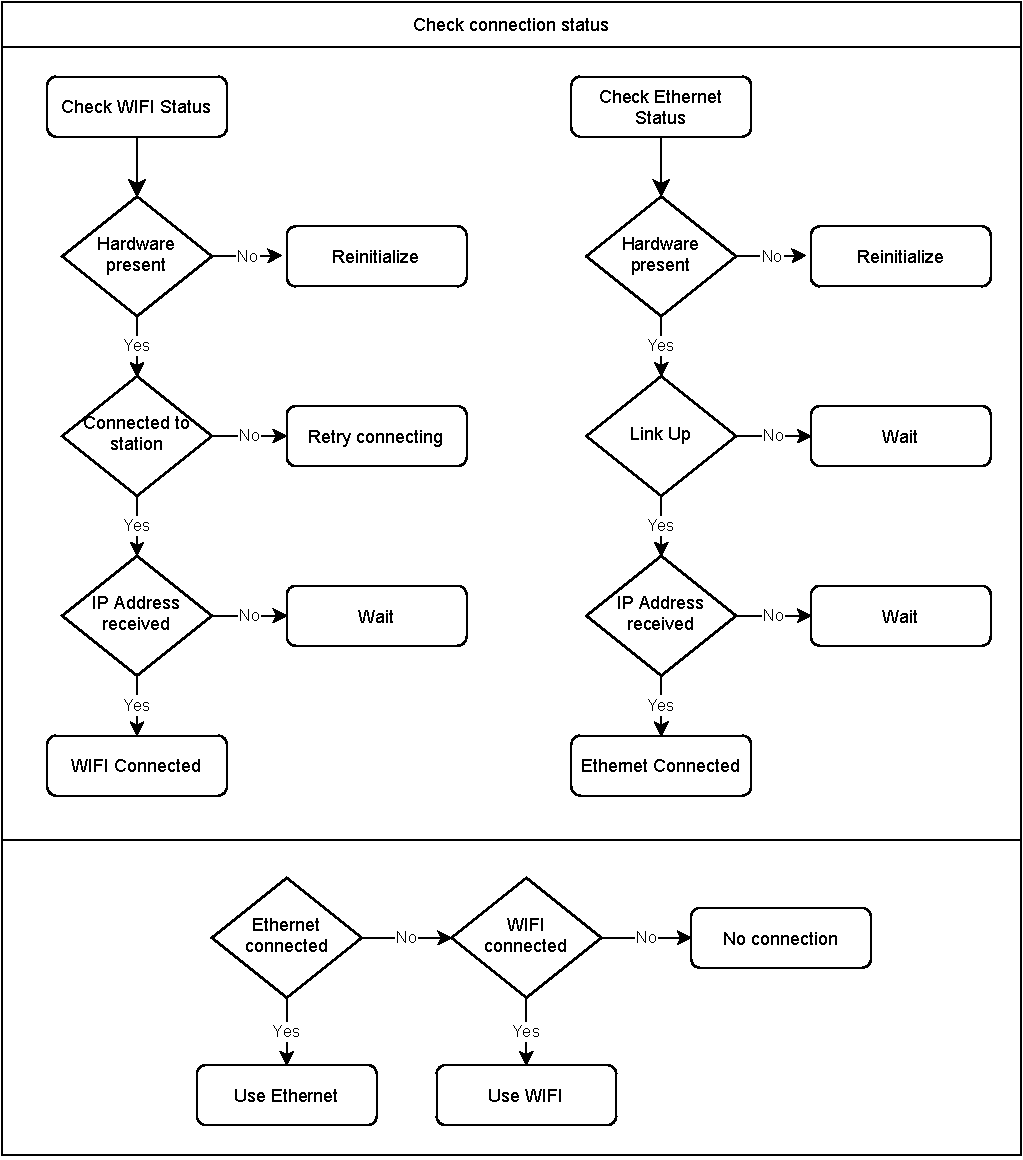
\includegraphics[height=14.5cm]{images/connection-tree}
	\caption{Flow chart of interface selection}
	\label{fig:connectin-tree}
\end{figure}
\newpage

\subsubsection{HTTP}
\acrfull{http} is used to communicate with the server and allows the Fleet-Monitor to read files and stream data. We decided to go with this technology because it is well supported by all libraries used. Data is transferred using HTTP POST requests containing data inside the body. The server response is used to check if the data was received correctly and validate the server connection. HTTP GET methods are used to read files from the server.

\subsubsection{Time synchronization}
In order for data to be useful it needs to have a timestamp. Ideally this timestamp would translate to a real time and date. This is why we implemented on both the server and client side a mechanism to synchronize the two. Every POST response from the server includes a JSON string with a field called Date. This field represents the current date and time and is used by the Fleet-Monitor to set its real time clock. Since the ESP32-S2 WROOM module does not have a dedicated oscillator for time keeping, the default 40 MHz crystal is used. The oscillator has a tolerance of ±10 \acrshort{ppm}. The maximum 24 hour drift can be calculated using the Equation \ref{eq:time}.
\medskip
\begin{equation}
\delta_{rel} =  \frac{1 s}{f} * \frac{f * \mathit{p}}{10^6} * t = \frac{1s}{40 MHz} * \frac{40 MHz * \pm10}{10^6} * 86400 s =  \pm0.864 s  
\label{eq:time}
\end{equation}

where:

\begin{conditions}
 f     &  frequency in Hz \\
 \mathit{p}     &  parts per million in \acrshort{ppm} \\
 t     &  time in s \\
\end{conditions}

Since this drift is quite large, we decided to update the real time clock of the ESP32 every 24 h to make sure both the server and the Fleet-Monitor always share the same time.

The timestamp is read out as $YYYY,MM,DD,hh,mm,ss$ and is stored locally in the \gls{unix} time format. 

\subsubsection{File Reload}
Additionally a mechanism was developed to automatically detect if a configuration file needs to be reloaded. A reload is needed when the file on the server was modified. Every HTTP POST response contains a JSON field called "ConfigReload". If this flag is set we will request the configuration file again from the server in order to clear the flag and get the newest configuration. The local configuration is then overwritten with the one from the server.

\newpage
\subsection{FMS Frames} \label{FMS Frame Handler}
Reading out frames from the CAN bus, filtering them and finally transmitting them to the server is done using two FreeRTOS tasks and a FreeRTOS queue. Figure \ref{fig:fms-software} illustrates this task view. The frame handler task has the highest priority as task switching while transmitting can cause issues.
\begin{figure}[h!]
	\centering
	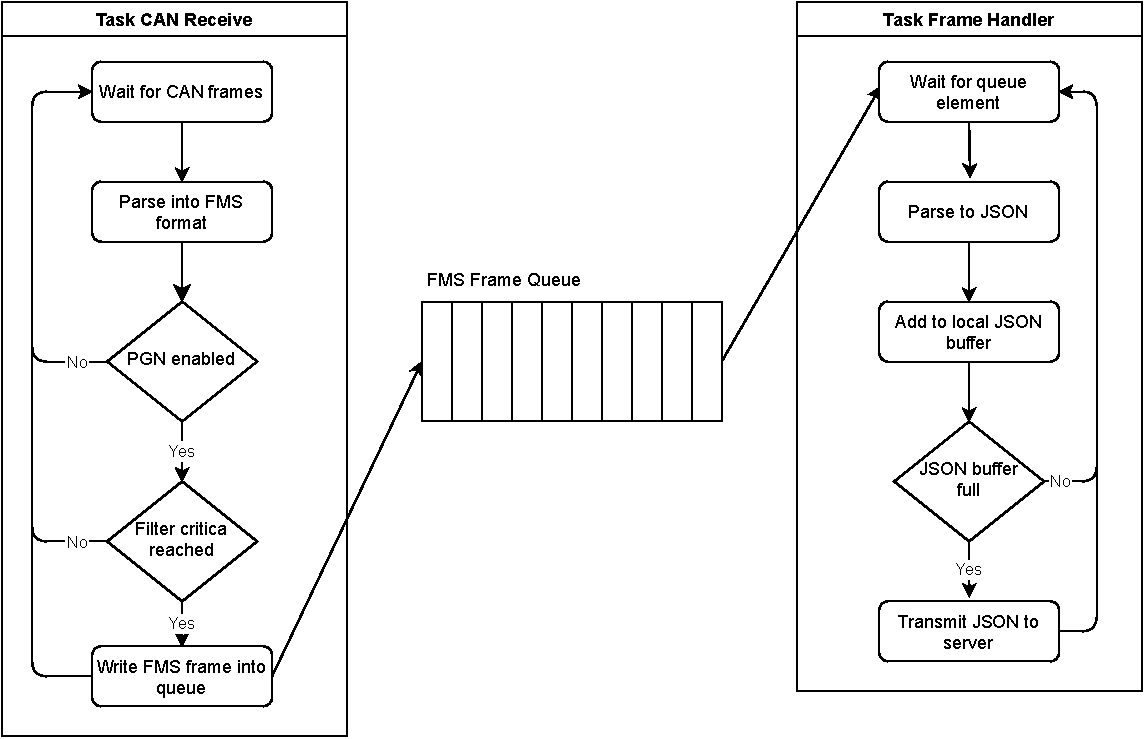
\includegraphics[width=\textwidth]{images/fms-software}
	%\vspace{0.0cm}
	\caption{FreeRTOS Tasks and Queue for FMS Frames}
	\label{fig:fms-software}
\end{figure}
\subsubsection{FMS Format Class}

\subsubsection{FMS Filter}
Both tasks will only start running once a configuration was read from either the server or from the local file system. The configuration is explained in the Section \ref{Frame Filter Configuration}.

Generally a frame can be enabled and disabled for the transmission, this helps remove unwanted packages from taking up valuable bandwidth. Additionally three filter methods were implemented to reduce the data rate and repetition of information:
\begin{itemize}
		\item On Change, data is only transmitted when something inside the data field of the frame changed. This is very useful for state supervision for example error codes, door states. 
		\item Interval, data is only transmitted with a set interval. Data in between the set interval is discarded. This filter method is used for things that are not very important but still good to know from time to time.
		\item No Filter, all the data received is being transmitted. This method is used for things that are very important to monitor.
\end{itemize}

\subsubsection{JSON Format}
A buffer is allocated to hold the FMS data from the queue, the data is parsed into JSON format

\begin{table}[h!]
    \begin{center}
    \framebox{
        \begin{tabular}{p{0.0cm} p{0.1cm} p{0.1cm} p{0.1cm} p{12.0cm}}                                     \\[-0.5em]
        & \multicolumn{3}{l}{$\triangledown$ \texttt{frames [n]}}                                        \\[0.3em]
        & & \multicolumn{2}{l}{$\triangledown$ \texttt{0 \{4\}}}                                          \\[0.3em]
        & & & \scalebox{0.8}{$\square$} \texttt{pgn:\;\ \quad\textbf{FEE9}}                               \\[0.3em]
        & & & \scalebox{0.8}{$\square$} \texttt{name:\;\quad\textbf{Fuel Consumption: LFC}}               \\[0.3em]
        & & \multicolumn{2}{l}{$\triangledown$ \texttt{1 \{4\}}}                                          \\[0.3em]
        & & & \scalebox{0.8}{$\square$} \texttt{pgn:\;\ \quad\textbf{FE6C}}                               \\[0.3em]
        & & & \scalebox{0.8}{$\square$} \texttt{name:\;\quad\textbf{Tachograph: TCO1}}                    \\[0.3em]
        \end{tabular}
    }
    \end{center}
%\vspace{-0.3cm}
\caption{\label{fig:frame-configuration-example}Frame Filter Configuration Example}
\end{table}
\newpage

\subsubsection{Transmission}
As already explained above in the Section \ref{Networking} data is being transmitted over the connected interface. If a request to the server times out or no confirmation is received, the JSON buffer is discarded. This is due to the amount of data gathered from the bus. The transmission body data length varies but is generally around 8000 bytes long.

\todo[inline]{Write about different filter settings as I mentioned it in section \ref{Frame Filter Configuration}}

\subsection{Accelerometer}
Luca


\newpage
\section{Utility Software Tools}
Several software tools have been write in python... \todo{Add more blabla}

\subsection{HTTP Server}
Luca

\newpage
\subsection{FMS Configuration Tool}
Changing the configuration of the \acrshort{fms}-Frame filter in a text editor is not very pleasing. Therefore a \acrfull{gui} has been developed to make this procedure easier and ensure a better overview of all settings. This tool is able to generate the \acrshort{json}-File structure as mentioned in Section \ref{Frame Filter Configuration}.

\subsubsection{Feature Description}
The configuration tool is decided into \textit{Global Settings} and \textit{Frame Settings}. The general options can be enabled or disabled by clicking on the corresponding checkbox. Further in the Frame Settings section, a table allows the user to change the filter settings of each \acrshort{fms}-Packet type. The filter features are described as followed:

\begin{description}
  \item[Active:] Enables or disables the transmission of this specific packet type
  \item[PGN:] Shows the \acrlong{pgn} in hexadecimal format \textit{(Read-Only)}
  \item[Name:] Shows the user friendly packet name \textit{(Read-Only)}
  \item[Filter:] Combo-box to select the filter type: \textit{No Filter}, \textit{On Change}, \textit{Max. Interval}
  \item[{Interval [ms]:}] Max. update rate, only available if filter type is set to: \textit{Max. Interval}
\end{description}

\medskip
\begin{figure}[h!]
	\centering
	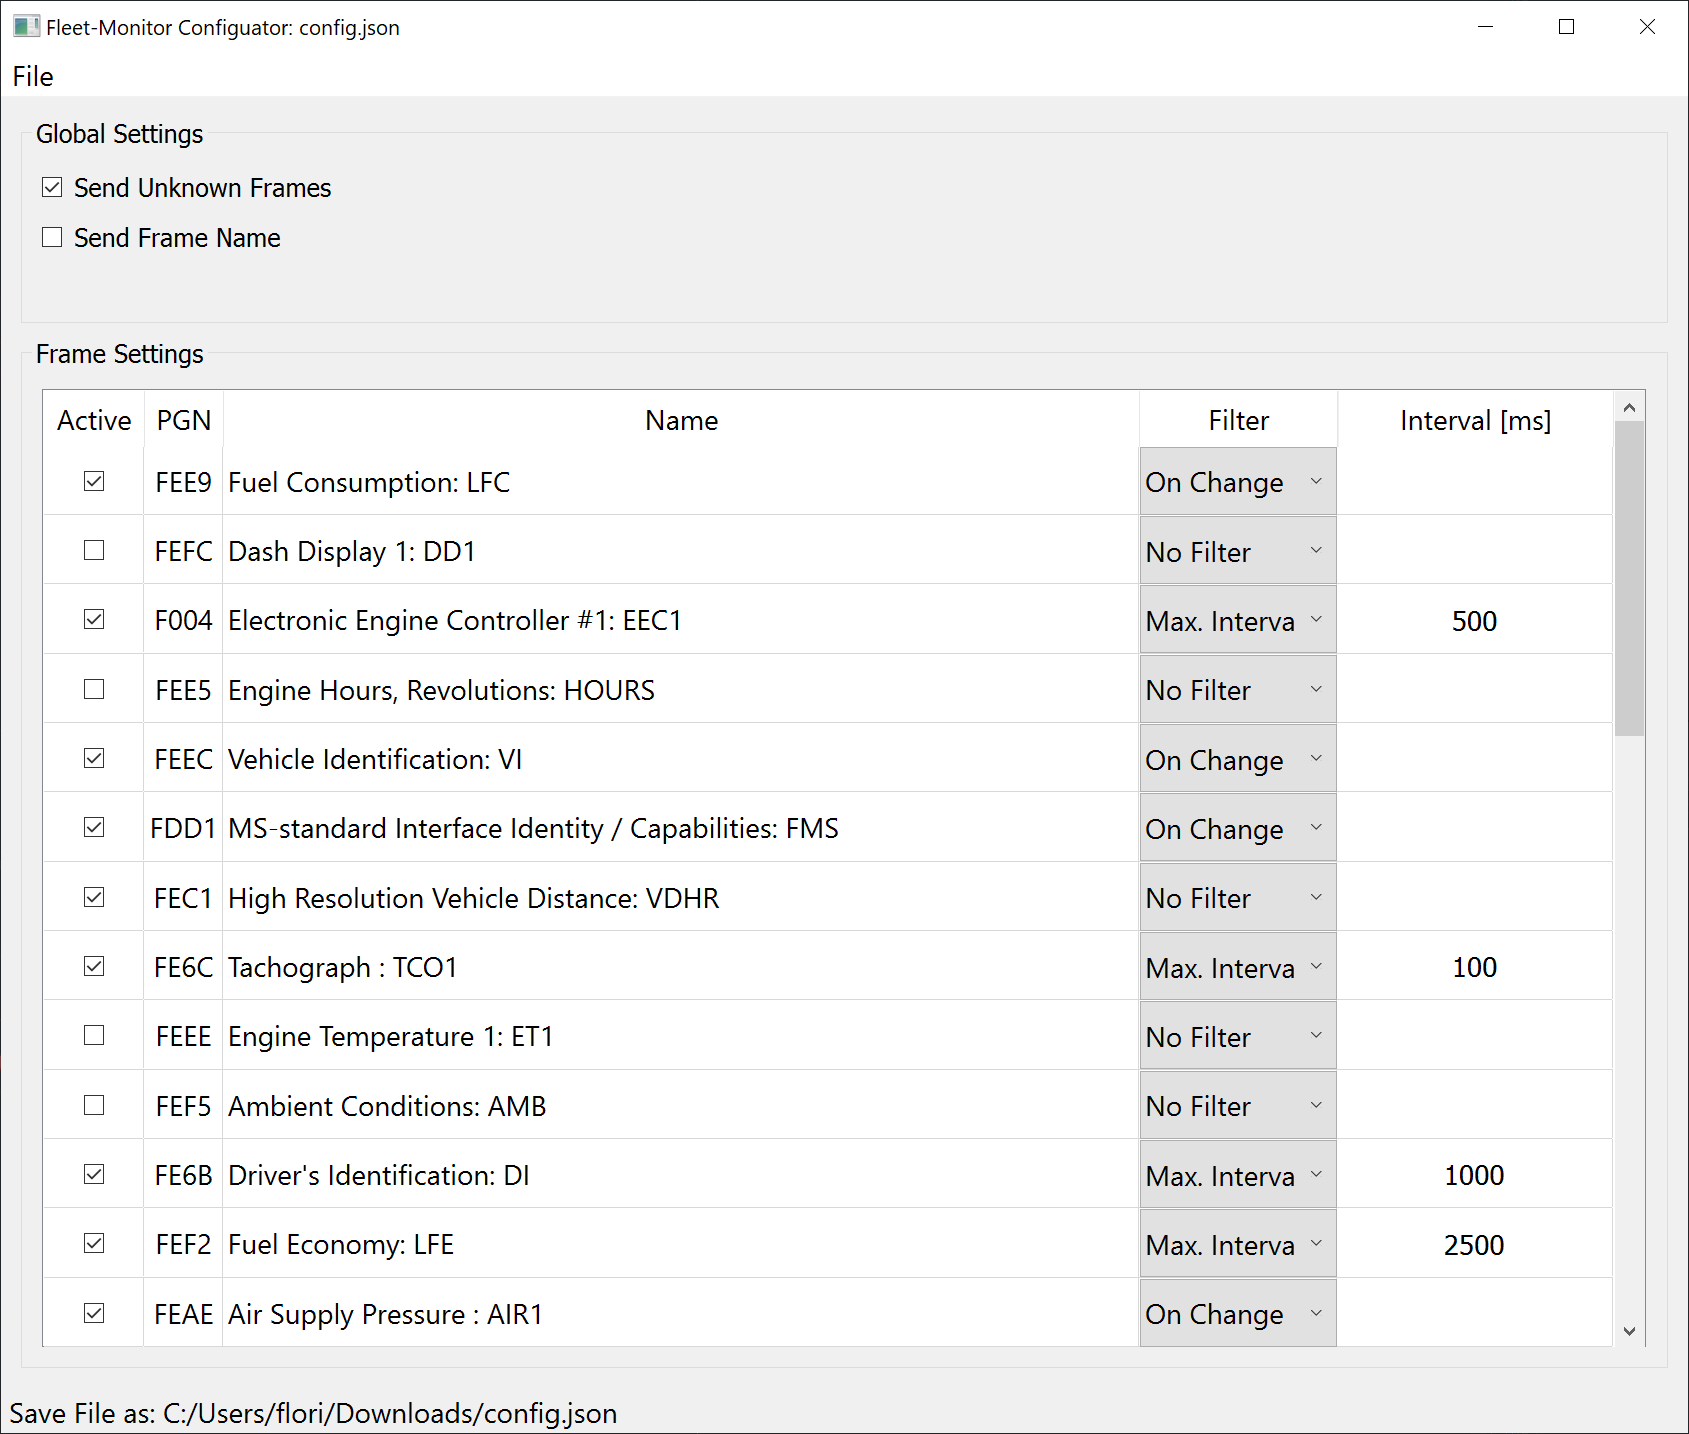
\includegraphics[width=\textwidth]{images/Configuration-Tool_Screenshot}
	\caption{FMS Frame Configuration Tool}
	\label{fig:configuration_tool}
\end{figure}
\newpage

\subsubsection{PyQt5}
As a framework

\subsubsection{File Loading \& Saving}
\begin{wrapfigure}{r}{4.0cm}
\vspace{-0.6cm}
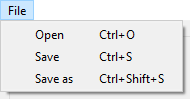
\includegraphics[width=4.0cm]{images/configuration-tool-file-panel}
\caption{File Menu-Bar}
\end{wrapfigure} 
To open an existing configuration file, three methods are available. Firstly via the menu-bar section, by clicking on the \textit{Open} button. Secondly by entering the keyboard shortcut \textit{Ctrl+O} and thirdly by dragging a file into the application. Saving files is very similar and intuitive due to the use of common shortcuts.
\newpage



\subsection{FMS Data Visualizer}
Flo 

\bigskip
\begin{figure}[h!]
	\centering
	\hfuzz=15.0pt
	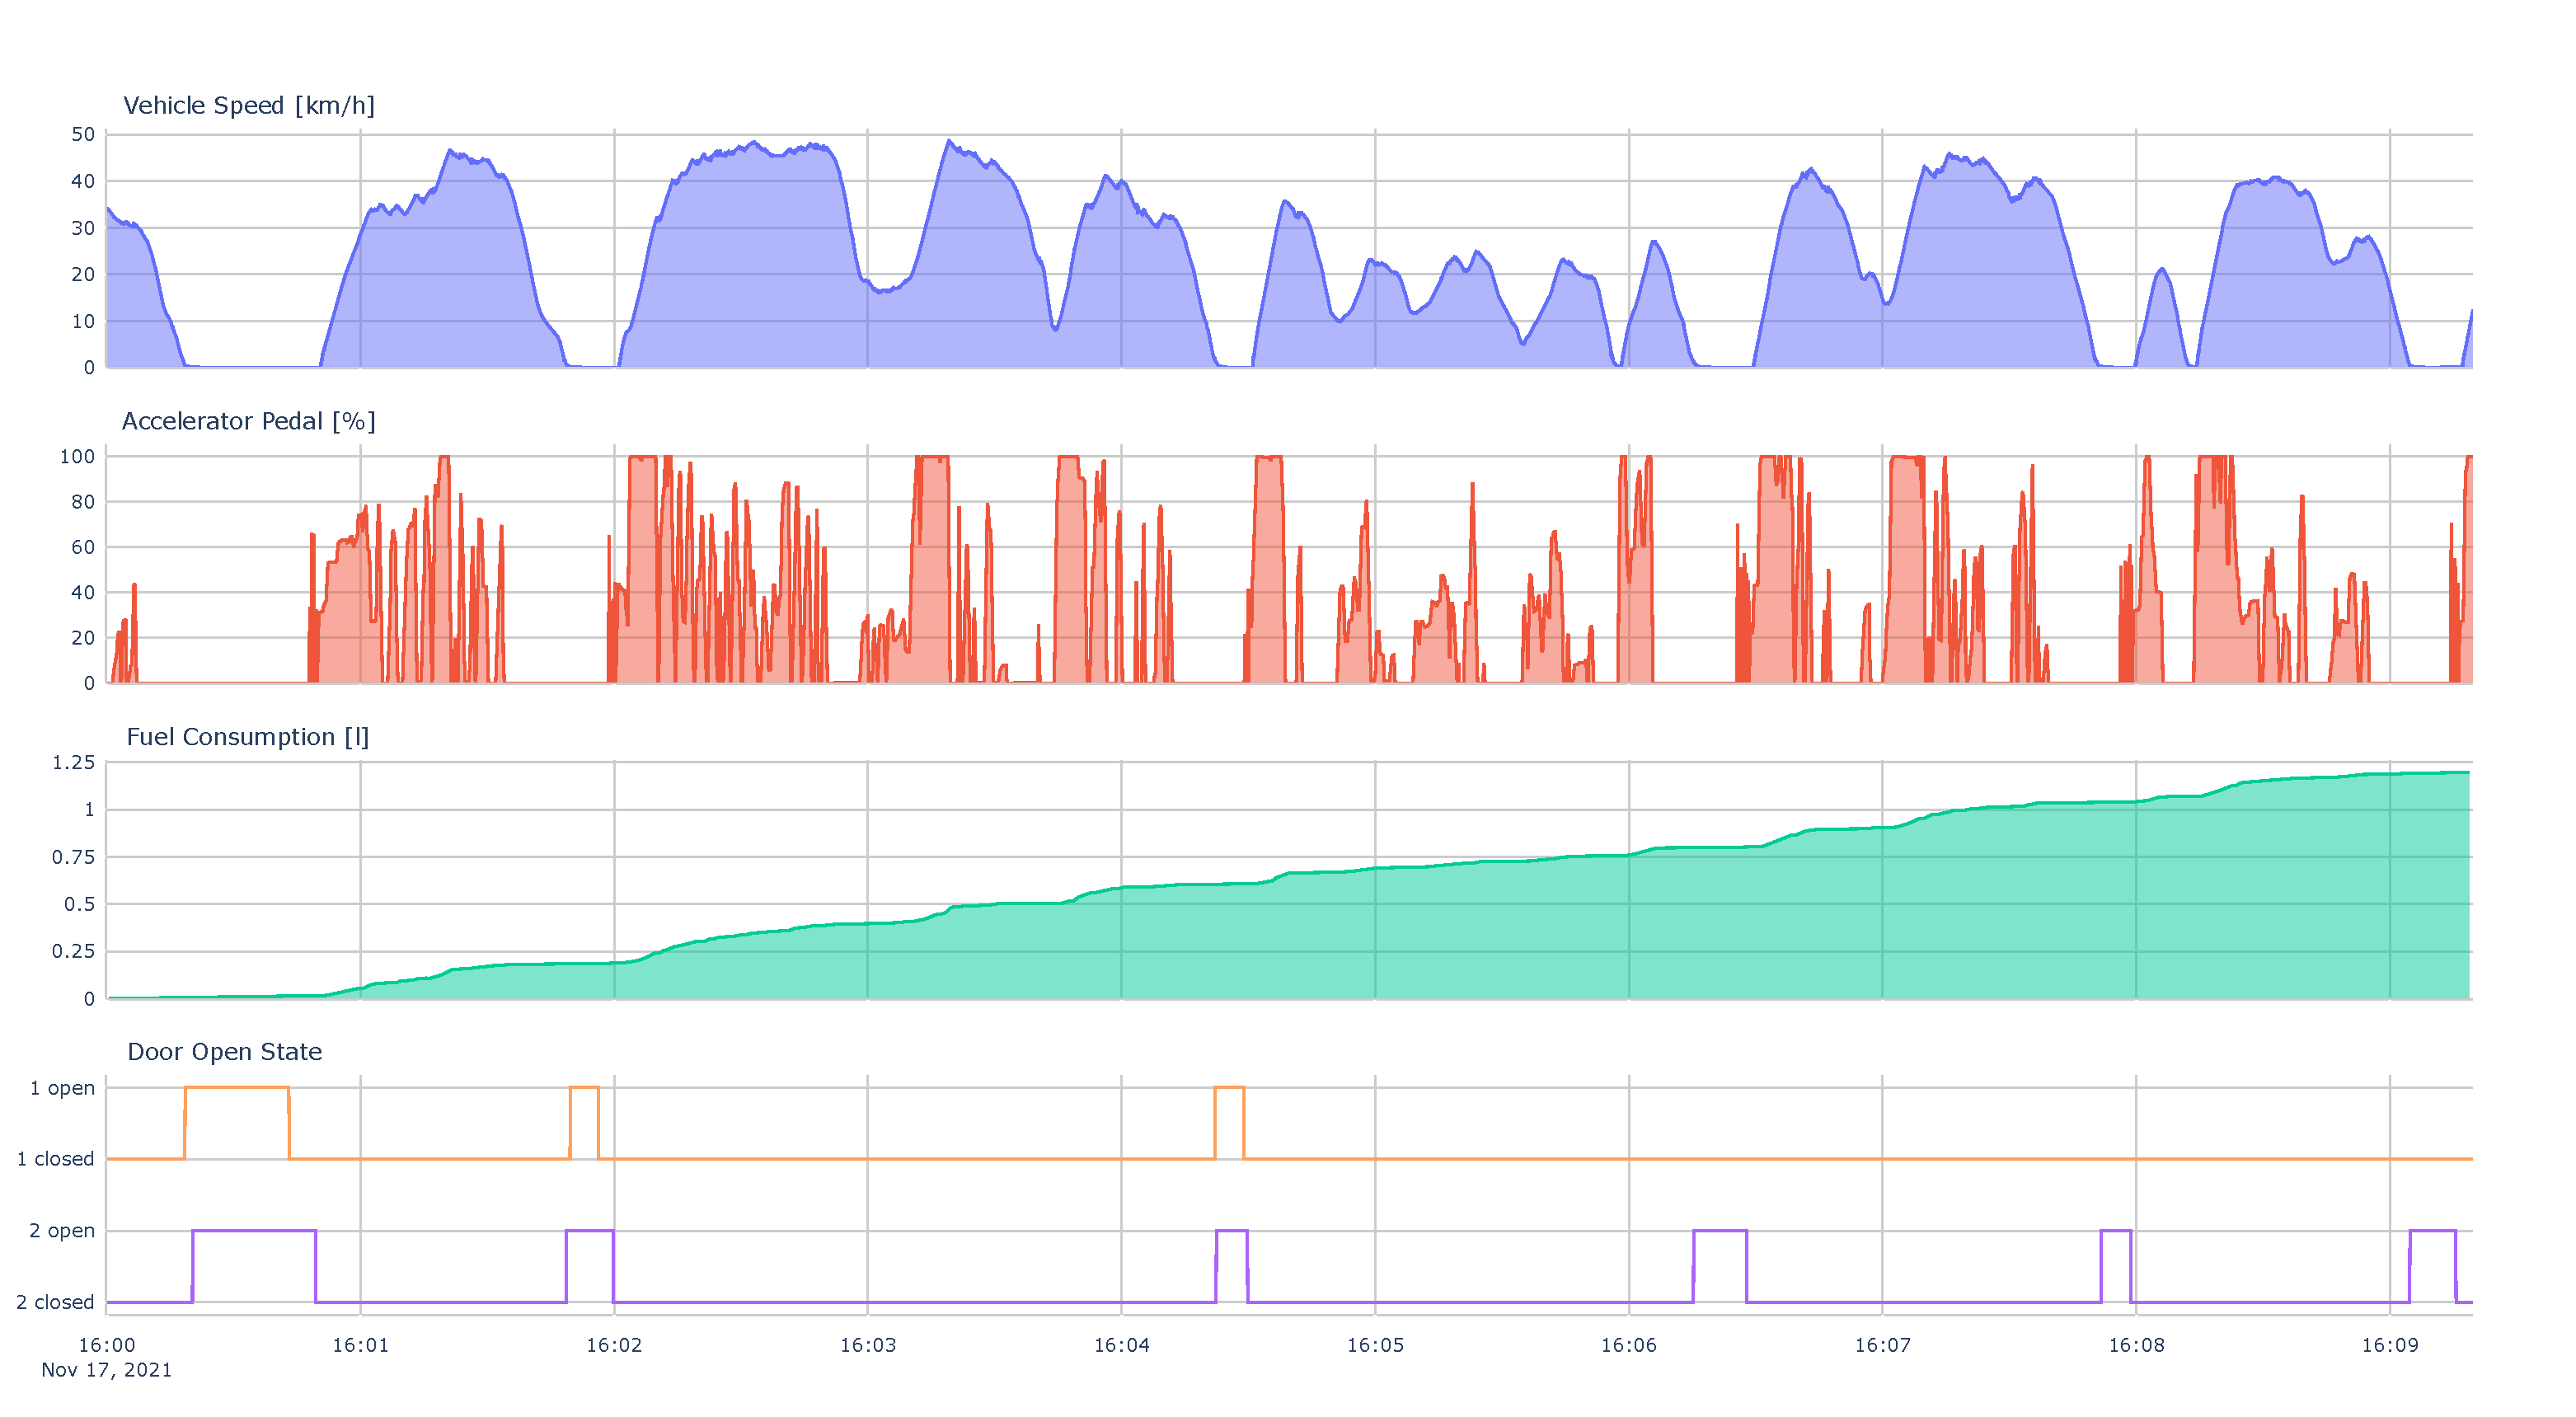
\includegraphics[width=15cm]{images/FMS_Data_Visualization.pdf}
	\caption{Visualization of FMS Data}
	\label{fig:fms_visualization}
\end{figure}
\newpage
